% Options for packages loaded elsewhere
\PassOptionsToPackage{unicode}{hyperref}
\PassOptionsToPackage{hyphens}{url}
\documentclass[referee,pdflatex,sn-basic]{sn-jnl}

\usepackage[T1]{fontenc}
\usepackage[utf8]{inputenc}
\usepackage{xcolor}
\usepackage{amsmath,amssymb,amsfonts}
\usepackage{longtable}
\usepackage{booktabs}
\usepackage{array}
\usepackage{multirow}
\usepackage{wrapfig}
\usepackage{float}
\usepackage{colortbl}
\usepackage{pdflscape}
\usepackage{threeparttable}
\usepackage{threeparttablex}
\usepackage[normalem]{ulem}
\usepackage{makecell}

% sn-jnl wraps every table float in threeparttable. The manuscript tables are
% generated by kableExtra, which already supplies that environment and may put
% it inside resizebox. Restore the original float environments saved by the
% class to avoid an illegal nested threeparttable while preserving Springer
% typography elsewhere.
\makeatletter
\renewenvironment{table}[1][]{\tableorg[#1]}{\endtableorg\normalfont}
\renewenvironment{sidewaystable}[1][]{\sidewaystableorg[#1]}{\endsidewaystableorg\normalfont}
\makeatother

\setcounter{secnumdepth}{3}

\usepackage{longtable,booktabs,array}
\usepackage{calc} % for calculating minipage widths
% Correct order of tables after \paragraph or \subparagraph
\usepackage{etoolbox}
\makeatletter
\patchcmd\longtable{\par}{\if@noskipsec\mbox{}\fi\par}{}{}
\makeatother
% Allow footnotes in longtable head/foot
\IfFileExists{footnotehyper.sty}{\usepackage{footnotehyper}}{\usepackage{footnote}}
\makesavenoteenv{longtable}
\usepackage{graphicx}
\makeatletter
\newsavebox\pandoc@box
\newcommand*\pandocbounded[1]{% scales image to fit in text height/width
  \sbox\pandoc@box{#1}%
  \Gscale@div\@tempa{\textheight}{\dimexpr\ht\pandoc@box+\dp\pandoc@box\relax}%
  \Gscale@div\@tempb{\linewidth}{\wd\pandoc@box}%
  \ifdim\@tempb\p@<\@tempa\p@\let\@tempa\@tempb\fi% select the smaller of both
  \ifdim\@tempa\p@<\p@\scalebox{\@tempa}{\usebox\pandoc@box}%
  \else\usebox{\pandoc@box}%
  \fi%
}
% Set default figure placement to htbp
\def\fps@figure{htbp}
\makeatother
\setlength{\emergencystretch}{3em} % prevent overfull lines
\providecommand{\tightlist}{%
  \setlength{\itemsep}{0pt}\setlength{\parskip}{0pt}}
\theoremstyle{thmstylethree}
\newtheorem{modelproposition}{Proposition}
\newtheorem{modelcorollary}{Corollary}
\newtheorem{modellemma}{Lemma}
\let\proposition\modelproposition
\let\endproposition\endmodelproposition
\let\corollary\modelcorollary
\let\endcorollary\endmodelcorollary
\let\lemma\modellemma
\let\endlemma\endmodellemma
\newcommand{\pospart}[1]{\left[#1\right]_{+}}
\usepackage{booktabs}
\usepackage{longtable}
\usepackage{array}
\usepackage{multirow}
\usepackage{wrapfig}
\usepackage{float}
\usepackage{colortbl}
\usepackage{pdflscape}
\usepackage{tabu}
\usepackage{threeparttable}
\usepackage{threeparttablex}
\usepackage[normalem]{ulem}
\usepackage{makecell}
\usepackage{xcolor}
\usepackage{bookmark}
\IfFileExists{xurl.sty}{\usepackage{xurl}}{} % add URL line breaks if available
\urlstyle{same}
\hypersetup{
  pdftitle={The Foreign Policy Impact of Trade-Based Status Gains: When China Overtakes the US as Top Export Destination},
  pdfkeywords={China, foreign policy alignment, international political economy, trade-based status, synthetic difference-in-differences, United Nations General Assembly},
  hidelinks,
  pdfcreator={LaTeX via pandoc}}

% Keep paragraph spacing stable in the double-spaced referee layout. The
% Springer class's flush-bottom setting can otherwise stretch vertical glue
% dramatically on pages with floats or short final paragraphs.
\setlength{\parindent}{1.5em}
\setlength{\parskip}{0pt}
\raggedbottom

\begin{document}

\title[Trade-Based Status Gains and Foreign Policy]{The Foreign Policy Impact of Trade-Based Status Gains: When China Overtakes the US as Top Export Destination}

% Author information intentionally omitted for double-anonymous review.

\abstract{\begin{singlespace}\textbf{Purpose:} How do countries adjust their foreign policy when a rising power becomes their leading trading partner?\\
\textbf{Methods:} I develop a formal model in which public recognition increases the salience of a new trade rank, and political leadership's cost-benefit analysis of foreign-policy alignment with the rising power determines its direction of change. To test the hypothesis derived from the model, I leverage the timing of China's surpassing the United States as Brazil's largest export destination and fit a synthetic difference-in-differences model to estimate the effect of the status change on Brazil's voting at the United Nations General Assembly. To assess whether the pattern extends beyond Brazil, I estimate a latent factor model using a cross-country panel for 2000-2022.\\
\textbf{Results:} Brazilian policymakers invoked China's new position to justify greater proximity between the countries, with voting convergence particularly visible on human rights issues. Relative to the counterfactual, the estimated reduction in bilateral voting distance is equivalent to 42 percent of the pre-treatment mean distance. The cross-country results are mixed, but interpreted as consistent with the model.\\
\textbf{Conclusion:} Publicly acknowledged changes in economic rank can support diplomatic adjustments in multilateral institutions, with implications for U.S.-China rivalry as their relative commercial positions change.\end{singlespace}}

\keywords{China, foreign policy alignment, international political economy, trade-based status, synthetic difference-in-differences, United Nations General Assembly}

\maketitle



\pagebreak

\section{Introduction}\label{introduction}

``China overtakes US as Brazil's top trade partner.'' That was a headline in many Brazilian newspapers in 2009 \citep{rodrigues2009}. The BBC ran a similar headline in 2021, when China surpassed the United States as the EU's biggest trading partner \citep{bbc2021}. During a high-profile trip to Beijing with an unusually large business delegation, President Lula da Silva invoked the milestone by noting that China was Brazil's largest export destination \citep{lula2009}.

Export statistics are updated monthly, and international trade journalists, diplomats, and policymakers follow them closely, so there is no new information being transmitted when one partner moves up the ladder of trade hierarchy. And yet, public discourse revolves around such categorical milestones. Why can a milestone, such as China becoming the number-one trade partner, matter politically despite adding little new information about the economic trend itself?

If everyone is perfectly rational, redundant information should not matter. Most of the literature on the effects of interdependence implicitly or explicitly assumes this hyperrationalist perspective and studies how trade and other economic ties shape foreign policy \citep{flores-macias_kreps2013, urdinez_etal2016, kastner_pearson2021}. Therefore, foreign-policy alignment should move gradually with trade exposure and economic interdependence in general. There is no expectation that discrete changes in economic or trade status will produce any effect on the foreign policy of countries.

Domestic political accounts of foreign policy, on the other hand, can conceivably attribute foreign-policy change to discrete changes, but only to changes such as new leadership ideology or political coalition \citep{neto2011, neto_malamud2015, rodrigues2019measuring, schenoniMythsMultipolaritySources2022}.

A different concern for the study of the effect of status change is reverse causality, since politically aligned countries may deepen economic ties with one another, making China's rise in the trade hierarchy a consequence rather than a cause of prior diplomatic affinity \citep{gowa1995, davis_pratt2021, struver2016}. If alignment reflects only accumulated exposure, domestic political reorientation, or prior diplomatic affinity, however, no specific symbolic milestone, such as becoming a top trade partner, should matter.

I argue that such milestones matter because they mark trade-based status gains. The argument builds on research that treats status as socially recognized standing within international hierarchies, clubs, and local status orders \citep{paul_larson_wohlforth2014, wolfRespectDisrespect2011, duque_2018, renshon2017, gotz_2021, roren_2024, roren2025_power_recognition, wolfTakingInteractionSeriously2019}. By trade-based status, I mean the recognized standing of a foreign power within a country's hierarchy of economically consequential relationships. Trade volume is continuous, but status is categorical: a partner can move from being important to being understood as central. Once that reclassification becomes public, the relationship is no longer merely larger than before. It becomes easier for political actors to invoke as a national priority, to defend as strategically consequential, and to use as a justification for diplomatic adjustment.

Much of the China and rising-powers branch of this literature asks how rising states seek recognition, major-power status, or institutional standing, and how misrecognition can produce contestation or revisionism \citep{deng2008_status, larson_shevchenko2010_status_seekers, ward2017_status_challenge, murray2018_recognition, mukherjee2022_ascending}. This argument relocates status from the ambitions of the rising power to the recognition practices of states. China's trade-based status gain occurs when another country publicly recategorizes China within its own hierarchy of external economic relationships -- from an important partner to a central one.

The argument links US-China competition to the recognition practices of third countries. When China overtakes the United States in a national trade hierarchy, its commercial rise can become a public basis for selective diplomatic accommodation. Multilateral voting provides an arena in which countries such as Brazil can adjust their positions toward China while retaining flexibility in other areas of foreign policy. This perspective locates one possible consequence of China's rise for the US-led international order in changes in diplomatic support within existing institutions.

I formalize the argument using a model with two players: political leadership and bureaucracy. The former chooses the foreign policy directive, and the latter decides to implements it. The leadership has sparse attention, and a public cue increases salience; as a result, it increases the weight of the costs and benefits of aligning with the emerging power. The model shows that the public cue is necessary for the new status to have an effect and that foreign policy change also depends on the ideological dispositions of political leadership.

Brazil is the strongest case for the theory. First, China displaced the United States, a politically salient incumbent, hegemonic benchmark, and the most important trade partner of Brazil for almost 80 years. Second, the rank reversal was publicly visible. Third, the Brazilian press allows the attention implication to be measured. The case is also substantively important because Lula-era Brazilian foreign policy is often described through autonomy, South-South activism, multipolarity, and Brazil's triangular position between the United States and China \citep{neto2011, neto_malamud2015, rodrigues2019measuring, schenoniMythsMultipolaritySources2022, guilhon2014, schenoni_leiva2021, brun_covarrubias2024, coutinho_rodriguez2024}.

To estimate the Brazilian foreign-policy alignment pattern, I use Synthetic Difference-in-Differences (SDiD) on annual UNGA ideal-point distance to China, with 2009 marking China's rise to the largest Brazilian export destination. UNGA voting is a standard measure to study alignment with China and other powers, linking votes to bilateral ties, ideology, sanctions, aid, Belt and Road membership, arms transfers, or Chinese economic returns \citep{potrafke2009, dreher_jensen2013, struver2016, yan_zhou2021, garcia_herrero_etal2024, steinert_weyrauch2024, he_zheng_chen2025, lektzian_biglaiser2023}.

In the preferred specification, the estimated reduced-form effect of when China became Brazil's largest export destination is a reduction of 0.273 ideal-point units in Brazil's distance to China relative to its synthetic counterfactual, equivalent to 42.2 percent of its pre-treatment mean, with a one-sided placebo-rank p-value of 0.031.

To assess whether a compatible directional pattern appears beyond Brazil and to check the narrower threat posed by explanations tied specifically to Brazil's 2009 calendar year, I extend the analysis to a cross-country panel in which China enters and holds the top goods-export destination position. The cross-country estimates are smaller in magnitude, consistent with a more heterogeneous sample, and point in the same direction as the Brazilian case. The pooled panel estimate is -0.101 (p-value = 0.010) and is stable across duration thresholds and sample restrictions (p-value between 0.003 and 0.019). The panel evidence identifies a directional pattern associated with entry into the goods-only rank condition; the public-status mechanism is measured directly only in the Brazilian case.

The paper's contribution is to show that economic status matters and impacts foreign policy. Existing work usually treats trade exposure as a smooth source of influence. I argue that accumulated trade growth can become politically consequential when it crosses a durable, publicly legible rank threshold. It is particularly likely when a great power, such as China, holds the new status. In the case of Brazil, China's rise to the top export destination position made an already expanding commercial relationship available in public and official language as evidence of China's new centrality. The mechanism evidence shows that the public cue was available and used by policymakers in their political discourse, working as a focal point.

The next section develops the status-threshold argument and derives observable implications. I then present the Brazil SDiD design and timing diagnostics, followed by issue-area and media evidence on the mechanism. The final empirical section evaluates whether durable China-top goods-export status is associated with similar movement in a broader cross-country panel.

\section{Theory and Hypotheses}\label{theory-and-hypotheses}

To explain the proposed mechanism and hypothesis, I present a simple formal model of sparse attention of policymakers \citep{gabaix2014}. I use sparsity to induce a symbolic cue effect that works as a public cue for foreign policy change.

\subsection{A simple model of public status cues}\label{a-simple-model-of-public-status-cues}

I model how political leadership chooses a policy directive and a diplomatic bureaucracy decides whether to implement it following a publicized change at the top of a country's trade ranking. Public recognition raises attention to the relationship and the bureaucracy's benefit from implementation. The leadership's evaluation of the relationship determines the direction of any policy response.

Let \(R\in\{0,1\}\) indicate whether a revisionist power occupies the top position in the relevant trade hierarchy for a given country. Let \(P\in\{0,1\}\) indicate whether that position has become publicly visible, for example, through press coverage using explicit ranking language.

I assume that policymakers' attention is sparse \citep{gabaix2014}. This means that a change in the new power's status competes for attention with other events in the world and does not automatically produce a change in foreign policy. I call the product \(q=RP\in\{0,1\}\) a political cue. It captures a situation in which the emerging power not only attains its new rank but also has that rank explicitly brought to public attention by the media or public officials. Let salience \(s(q)\geq0\) satisfy \(s(1)>s(0)\). In words, becoming the new number one and receiving public recognition makes the emerging power more salient to policymakers, bringing it to their attention. The function \(s(q)\) represents this attention as an exogenous decision weight.

\subsubsection{Valence}\label{valence}

Let:

\begin{itemize}
\tightlist
\item
  \(G\geq0\): the baseline perceived gains from moving closer to the new great power;
\item
  \(D\geq0\): the baseline perceived costs of increased dependence on the emerging power;
\item
  \(\iota\in[-1,1]\): the leadership's ideological orientation toward the emerging power, where
\end{itemize}

\[
\begin{cases}
\iota>0 & \text{indicates a favorable view of the emerging power;}\\
\iota=0 & \text{indicates neutrality;}\\
\iota<0 & \text{indicates an unfavorable view of the emerging power.}
\end{cases}
\]

The quantities \(G\) and \(D\) are evaluated on a common utility scale before ideological weighting. Ideology affects how much importance the leadership assigns to each component. I define the net marginal value of strengthening ties with China as

\[
\theta=(1+\iota)G-(1-\iota)D
      =(G-D)+\iota(G+D).
\]

An ideologically neutral leadership, \(\iota=0\), evaluates the relationship according to \(G-D\). A favorable orientation increases the weight on gains and reduces the weight on dependence costs; an unfavorable orientation does the reverse. Both weights are nonnegative and sum to two. At the endpoints, \(\iota=1\) places zero weight on dependence costs and \(\iota=-1\) places zero weight on gains. Thus ideology operates through the evaluation of the relationship: if \(G=D=0\), then \(\theta=0\) for every ideological orientation.

Positive \(\theta\) makes movement toward China attractive before adjustment costs; negative \(\theta\) favors hedging or distancing. When \(G+D>0\), the evaluation equals zero at \(\iota_0=(D-G)/(G+D)\). For example, with \(G=2\) and \(D=5\), an orientation of \(\iota=0.5\) yields \(\theta=0.5\), whereas \(\iota=-0.5\) yields \(\theta=-6.5\). Whether either evaluation produces an actual policy change also depends on the costs and implementation conditions specified below. The comparison between \(q=0\) and \(q=1\) holds \(G\), \(D\), and \(\iota\) fixed.

\subsubsection{Players, actions, and information}\label{players-actions-and-information}

There are two players:

\begin{enumerate}
\def\labelenumi{\arabic{enumi}.}
\item
  The political leadership, \(L\), chooses a policy directive \(d\in\mathbb{R}\), measured as a normalized adjustment relative to the existing policy. Positive values indicate movement toward China; negative values indicate hedging or distancing. A directive of \(d=0\) preserves the existing policy.
\item
  The diplomatic bureaucracy, \(B\), observes the directive and chooses \(e\in\{0,1\}\), where \(e=1\) means implementation.
\end{enumerate}

The realized policy is

\[
y=ed.
\]

The baseline model assumes complete information: \(q\), \(G\), \(D\), \(\iota\), the salience and implementation-benefit functions, and the costs are common knowledge.

\subsubsection{Timing and payoffs}\label{timing-and-payoffs}

The game proceeds in the following order:

\begin{enumerate}
\def\labelenumi{\arabic{enumi}.}
\item
  The leadership chooses the directive \(d\).
\item
  The bureaucracy observes \(d\) and chooses \(e\).
\item
  The policy \(y=ed\) is realized, and payoffs are received.
\end{enumerate}

The leadership values policy changes that move the relationship in its preferred direction, but must weigh that return against the costs of departure from existing policy. Its payoff, normalized to zero when it issues no directive, is

\[
u_L(d,e;q)
=
e\left[s(q)\theta d-\frac{d^2}{2}\right]
-c_L|d|,
\tag{1}
\]

The term \(s(q)\theta d\) captures the perceived return from the direction and extent of an implemented adjustment. For positive salience, movement toward China yields a positive return when \(\theta>0\); when \(\theta<0\), a negative directive yields a positive return by moving away from a relationship the leadership evaluates unfavorably. Salience determines the weight this evaluation receives in the policy decision. A public cue can therefore increase the incentive to act in either direction while leaving the underlying evaluation \(\theta\) unchanged.

The quadratic term \(d^2/2\) captures the increasing marginal cost of larger implemented departures from existing policy, such as the disruption involved in revising established commitments. Its curvature is normalized to one for simplicity. This term limits the preferred extent of adjustment even when the leadership strongly favors a particular direction. The factor \(e\) multiplies both this cost and the directional return because they arise only when the bureaucracy carries out the directive.

By contrast, \(c_L|d|\), with \(c_L>0\), captures the political effort and reputational exposure involved in formulating and defending a directive, whether or not it is implemented. For example, proposing a change in diplomatic voting instructions requires articulating and defending the new position even if the bureaucracy subsequently leaves voting practice unchanged. This cost rises with the size of the proposed departure and applies to both directions. Conditional on implementation, it creates a region of inaction: the leadership issues a nonzero directive only when the initial marginal return \(s(q)|\theta|\) exceeds \(c_L\).

The bureaucracy's payoff, with \(c_B>0\), is

\[
u_B(e,d;q)
=
e\,\mathbf{1}\{d\neq0\}\,[K(q)-c_B],
\tag{2}
\]

The bureaucracy derives no utility from moving closer to China or to the United States, \(K(q)\) represents the benefits of implementing a given policy, and \(c_B\) the costs. When deriving the equilibrium, I also assume that \(K(1)>K(0)\), which means that implementing a public policy generates higher benefits than a policy without a public cue.

\subsubsection{Equilibrium}\label{equilibrium}

The solution concept is subgame-perfect equilibrium, obtained by backward induction.

\modellemma[Bureaucratic response]
For any directive $d\neq0$, the bureaucracy implements if and only if $K(q)>c_B$. In the event of equality, the conservative tie-breaking rule $e=0$ applies.
\endmodellemma

\textit{Proof.} If \(d\neq0\), implementation yields \(K(q)-c_B\), whereas non-implementation yields zero. Comparing the two directly gives the condition. If \(d=0\), there is no policy to implement, and \(e=0\) is adopted. \(\square\)

\modelproposition[Equilibrium with a directionally neutral cue]
The policy outcome in the subgame-perfect equilibrium is

\[
y^*(q)=
\mathbf{1}\{K(q)>c_B\}
\operatorname{sign}(\theta)
\left[s(q)|\theta|-c_L\right]_{+}.
\tag{3}
\]

where $\left[x\right]_{+}=\max\{x,0\}$. The leadership chooses $d^*(q)=y^*(q)$, anticipating the bureaucratic response specified in Lemma 1.

In particular, the cue can change whether a response occurs and how strong it is, but it does not determine its sign.
\endmodelproposition

\textit{Proof.} If \(K(q)\leq c_B\), the bureaucracy does not implement nonzero directives. Since the leadership pays \(c_L|d|\) even for a directive that is not implemented, its optimal choice is \(d=0\), and therefore \(y=0\).

\begin{minipage}{\linewidth}
If $K(q)>c_B$, every nonzero directive is implemented. The leadership solves

\[
\max_d\left\{s(q)\theta d-\frac{d^2}{2}-c_L|d|\right\}.
\]
\end{minipage}

For \(d>0\), the first-order condition is \(d=s(q)\theta-c_L\); this solution is positive only when \(s(q)\theta>c_L\). For \(d<0\), the condition is \(d=s(q)\theta+c_L\); it is negative only when \(s(q)\theta<-c_L\). In all other cases, the subgradient condition is satisfied at \(d=0\). Combining the three regions yields (3). \(\square\)

To complete the earlier example, take \(G=2\), \(D=5\), and \(\iota=0.5\), so \(\theta=0.5\). Let \(s(0)=0.5\), \(s(1)=1\), \(c_L=0.4\), \(K(0)=2\), \(K(1)=3\), and \(c_B=1\). These are hypothetical normalized values without empirical calibration. The bureaucracy would implement a nonzero directive in either state. Before the cue, \(s(0)|\theta|=0.25\leq0.4\), so \(y^*(0)=0\); after the cue, \(s(1)|\theta|=0.5>0.4\), so \(y^*(1)=0.5-0.4=0.1\).

\medskip

\noindent\textbf{Immediate implications.}

\modelcorollary[The cue has no intrinsic valence]
Whenever $y^*(q)\neq0$,

\[
\operatorname{sign}\bigl(y^*(q)\bigr)=\operatorname{sign}(\theta).
\]

A nonzero response moves toward China when $\theta>0$ and away from China when $\theta<0$; the latter may represent hedging or distancing.
\endmodelcorollary

\modelcorollary[Activation through attention or implementation incentives]
The cue activates a previously absent response when both post-cue conditions hold,

\[
K(1)>c_B
\quad\text{and}\quad
s(1)|\theta|>c_L,
\]

and at least one of them failed to hold before the cue:

\[
K(0)\leq c_B
\quad\text{or}\quad
s(0)|\theta|\leq c_L.
\]
\endmodelcorollary

\modelcorollary[Benchmark with unchanged attention and implementation benefits]
For this comparison, relax the strict assumptions $s(1)>s(0)$ and $K(1)>K(0)$ by setting $s(1)=s(0)$ and $K(1)=K(0)$. When the public label changes neither attention nor implementation benefits, the equilibrium policy remains unchanged.
\endmodelcorollary

The general result therefore concerns magnitude:

\[
|y^*(1)|\geq|y^*(0)|
\]

when the cue weakly increases \(s\) and \(K\). The direction depends on \(\theta\).

\subsubsection{Extensions}\label{extensions}

\medskip

\noindent\textbf{Issue-specific costs.}
To capture selective adjustment, let \(c_L=c_{Lk}\) and \(\theta_k=(1+\iota)G_k-(1-\iota)D_k\) for each issue \(k\), where \(G_k\) and \(D_k\) are the baseline gains and dependence costs relevant to that issue. Conditional on implementation being available both before and after the cue, the attention channel activates a previously absent response on issues satisfying

\[
s(0)|\theta_k|\leq c_{Lk}<s(1)|\theta_k|.
\]

Issues with an already active response can also adjust further as salience increases; issues whose costs remain above the post-cue threshold remain unchanged. If the cue instead makes implementation available for the first time, the activation conditions in Corollary 2 apply issue by issue. The composition of the response depends on the distribution of valuations and costs and does not follow automatically from an issue being classified as human rights or belonging to any other substantive area.

\medskip

\noindent\textbf{Persistence and incumbent prominence.}
Let \(\rho\) denote the expected persistence of the new hierarchy and \(h\) the prominence of the displaced partner. A simple extension allows

\[
\frac{\partial s(1;\rho,h)}{\partial\rho}>0,
\qquad
\frac{\partial s(1;\rho,h)}{\partial h}>0,
\]

with analogous relationships for \(K\). A persistent ranking provides a more stable basis for adaptation; displacing a prominent incumbent makes the reclassification more visible. Neither condition determines the valence of \(\theta\). Holding the leadership's evaluation and both players' costs fixed, increases in persistence or incumbent prominence that raise salience and implementation benefits weakly increase the absolute value of the post-cue policy response, subject to the same thresholds.

\subsection{Interpretation}\label{interpretation}

Policymakers must consider many factors when deciding to change foreign policy. These include trade statistics across many countries, GDP growth, shifts in the balance of power, new alliances and trade partnerships, new technologies, domestic politics, and more. A trade-based status shift may draw attention to a potential policy change that otherwise would not occur through smooth growth in economic interdependence. It simplifies complex economic relationships, helps elites coordinate attention \citep{bordalo_etal2022, conlon2023, enke2024, graeber_etal2025}, and serves as a focal point \citep{schelling1960}.

This attribution of symbolic status between two countries is a common feature of foreign policy. Leaders in Canada refer to their country as a middle power \citep{chapnick1999}. Churchill famously called the US-UK relationship a special one \citep{reynolds1985}. Mitterrand used ``couple franco-allemand'' to promote the European Union \citep{krotz_schild2013}. My argument is that trade status works similarly.

The mechanism has two steps. First, media coverage or official recognition of the new status makes China and the bilateral relationship more visible, increasing \(s(q)\). Second, greater attention from policymakers allows them to perceive a greater marginal net benefit, \(s(q)\theta\), of closer ties with the new major trade partner.

\subsection{Hypothesis}\label{hypothesis}

One would think that the main hypothesis would be that a public cue (by the media and/or political leadership) of a new trade status acquired by an emerging power should generate closer alignment toward that partner.

However, as the model makes clear, a public cue of the new status may instead induce a policy response in the opposite direction. A number-one status may create anxiety among political elites and prompt a decision to move further away from China rather than toward the expected alignment, because the perceived costs outweigh the benefits. It depends on the value of \(\iota\) in the model, which measures policymakers' favorability toward a foreign policy closer to China.

As a result, the hypothesis tested in the paper is: All else equal, whenever a political leadership is favorably oriented toward China (\(\iota>0\)), a public cue of a new trade status by an emerging power increases the probability of closer approximation toward that partner.

For Brazil, with a leftist government interested in South-South cooperation, I argue that the assumption of \(\iota>0\) is plausible. For other countries, the paper's assumption that they will view China favorably is plausible (though not certain) until the mid-2010s, when the US-China rivalry was not as intense as it became by the end of the decade.

Since I am estimating a reduced-form model, the mechanism is not estimated directly from the model. As mentioned, an increased public cue may not induce foreign-policy alignment toward China because a new directive also depends on the leadership's ideological leanings toward China. Another important caveat that the cross-country regression makes clear is that, without a public cue, the model predicts no foreign policy change as a result of the new trade status of the emerging power. Without systematic data on the presence or absence of public cues for every country, I may be mixing cases with and without a public cue. Thus, I expect the average effect to be smaller than in the Brazil case.

The model extension also implies a durability condition. The higher the persistence of the new status, the higher the salience, which should increase the likelihood of a foreign policy orientation. A one-year episode of China as the number one trade partner may attract attention, but it is a weaker treatment regime.

Last but not least, trade-based status changes may impact foreign policy issues differently. Some foreign-policy arenas are especially suitable for this kind of adjustment. There are two key conditions: the country and the newly elevated partner previously differed, and the costs of movement are high enough to prevent adjustment before the cue but low enough to be overcome afterward.

\section{Data and Design}\label{data-and-design}

The theoretical concept of interest is the rising power obtaining the status of top trade partner of a country. However, public status language varies in what counts as a top trade partner and in how it is described. Officials and journalists may describe China as the largest trading partner, main commercial partner, or top export market, for instance. Countries also value different things as a matter of status: largest flow of trade (exports plus imports) is what matters for some countries. For others, it is largest total exports (goods and services), or largest goods exports.

For the argument advanced in the article, what matters is the status change. Export-destination rank operationalizes the trade-based status shift. But since I have more information about Brazil than about other countries, I explain the differences in how I operationalize the treatment in the SDiD model and the cross-country panel regression.

\subsection{SDiD Design}\label{sdid-design}

In the design in which Brazil is the only treated country, the treatment is given by an export-destination rank in goods trade -- China becoming number one in that rank. In Brazil, public and official language tracks that rank: the 2009 coverage announcing that China had overtaken the United States as the country's largest trading partner was reporting precisely that change.

The primary outcome is absolute UNGA ideal-point distance to China, based on the annual ideal-point estimates of \citet{bailey_etal2017}. Lower values indicate convergence toward China. This measure is preferable to raw annual agreement shares for the main design because it is less sensitive to changes in the UNGA agenda over time. I use resolution-level agreement diagnostics only to interpret where convergence appears strongest. As a measurement-robustness check, the appendix re-estimates the main specifications using ideal points estimated by \citet{fjelstul_etal2026}, which are slightly different from \citet{bailey_etal2017} and based on another sample of resolution-related votes.

For Brazil, the treatment indicator equals one from 2009 onward, the first year China became Brazil's largest export destination. SDiD estimates Brazil's average post-2009 gap relative to a weighted synthetic counterfactual. Unit weights are learned from pre-treatment outcome histories, whereas the optimized pre-treatment time weights use control outcomes before onset and the controls' average outcome after onset \citep{arkhangelsky_etal2021}. The design is reduced-form. Its credibility rests on pre-treatment fit, rank-versus-volume timing tests, donor-pool sensitivity, and outcome robustness.

The SDiD panel combines UNGA ideal points with trade, macroeconomic, power, geographic, institutional, and trade-agreement variables. The complete panel covers 96 countries and 19 Brazil years for the main SDiD window (1997-2015). The preferred estimator uses no covariates: the counterfactual is built from pre-treatment outcomes together with the SDiD unit and time weights. Time-varying variables enter only comparison specifications. Trade data come from the International Trade and Production Database for Estimation \citep{borchert_etal2021}. The ITPD-E \texttt{trade} variable is measured in millions of current US dollars, and export-destination ranks are computed from exporter-importer flows.

The Brazil variables enter the design in three groups. The outcome is Brazil's annual absolute UNGA ideal-point distance to China; the treatment is an indicator for years after China becomes Brazil's largest export destination; and observed country characteristics are used for diagnostics and comparison specifications. The preferred counterfactual is driven by pre-treatment outcomes and SDiD unit and time weights, not by effective covariate adjustment. Contemporaneous trade, macroeconomic, power, ideology, and institutional measures remain available for comparisons but are not preferred because their post-2009 values may be mediators or outcomes of the same shocks.

The panel regression uses the same outcome but constructs treatment separately from goods-only export-destination ranks and a status-current risk set. Table \ref{tab:table-summary-main} summarizes the full country-year panel from which the Brazil specifications are constructed.

\begin{table}[H]
\centering
\caption{\label{tab:table-summary-main}Descriptive statistics for the country-year panel used in the Brazil SDiD design.}
\centering
\resizebox{\ifdim\width>\linewidth\linewidth\else\width\fi}{!}{
\fontsize{8}{10}\selectfont
\begin{threeparttable}
\begin{tabular}[t]{lccccc}
\toprule
Variable & N & Mean & SD & Min & Max\\
\midrule
Treatment & 1824 & 0.00 & 0.06 & 0.00 & 1.00\\
UNGA distance to China & 1824 & 0.91 & 0.80 & 0.00 & 4.22\\
UNGA distance to US & 1824 & 2.65 & 0.92 & 0.00 & 5.06\\
Geographic distance to US & 1824 & 0.00 & 0.50 & -1.14 & 1.11\\
Trade share with China & 1824 & -0.01 & 0.49 & -0.36 & 4.96\\
\addlinespace
Trade share with US & 1824 & 0.00 & 0.50 & -0.41 & 1.87\\
Power index & 1824 & 0.00 & 0.50 & -0.12 & 5.01\\
Power gap to US & 1824 & 0.03 & 0.49 & -3.90 & 0.43\\
GDP per capita & 1824 & -0.00 & 0.50 & -0.37 & 2.81\\
Exchange rate & 1824 & -0.00 & 0.49 & -0.15 & 6.82\\
\addlinespace
HoG left ideology & 1824 & 0.40 & 0.49 & 0.00 & 1.00\\
Current account & 1824 & 0.00 & 0.50 & -3.24 & 2.56\\
Government deficit & 1824 & 0.01 & 0.50 & -6.59 & 3.33\\
Parliamentary system & 1824 & 0.39 & 0.49 & 0.00 & 1.00\\
Military executive & 1824 & 0.11 & 0.31 & 0.00 & 1.00\\
\addlinespace
US trade agreement & 1824 & 0.09 & 0.28 & 0.00 & 1.00\\
\bottomrule
\end{tabular}
\begin{tablenotes}
\item \textit{Note: } 
\item Country-year variables from the SDiD analytic panel; continuous covariates are rescaled in the estimation data, UNGA distances are ideal-point distances, and treatment is binary. Window: 1997-2015 SDiD analytic panel. Observations include Brazil and donor countries used to construct the synthetic counterfactual. The treatment mean is small because only Brazil is treated after 2009. Covariate summaries describe the full analytic panel; the preferred estimate uses none of them.
\end{tablenotes}
\end{threeparttable}}
\end{table}

\subsection{Identification Strategy}\label{identification-strategy}

I want to estimate the causal effect of China rising to first place among a country's export destinations on its foreign policy. The main direct challenge to causal identification is differentiating it from a continuous foreign-policy approximation as exposure to trade with China increases over time. Besides that, countries may move closer to China due to changes in domestic political coalitions or foreign-policy doctrine reorientation that coincide in timing with the treatment, because governments already inclined toward China deepen commercial ties before the rank reversal occurs, or due to any other confounding variable.

To address these issues, I use Synthetic Difference-in-Differences (SDiD). Like the Synthetic Control Method (SCM), it constructs a weighted counterfactual from a donor pool to estimate the causal effect, using weights to approximate the counterfactual in ways that DiD cannot. Unlike the SCM and similar to the DiD, it estimates unit fixed effects, but with different weights. This combines both methods into a single one. As a result, violations of (unweighted average) parallel trends do not mean violations of weighted parallel trends. It also weights pre-treatment periods so that the controls' weighted pre-treatment outcomes approximate their average post-treatment outcomes. In other words, the weights pool observations to reduce bias in a latent factor model, even when global parallel trends are not valid. \citet{arkhangelsky_etal2021} show SDiD is consistent under this latent factor model when weights converge adequately.

The preferred specification uses no covariates because time-varying post-2009 values may induce post-treatment bias. The current-covariate comparison passes the country-year variables listed in Table \ref{tab:outcome-robustness-table} to \texttt{synthdid}; its continuous inputs are rescaled separately, while indicator variables retain their coding. Geographic distance to the United States is time-invariant: it remains in the comparison array but is absorbed by the unit-effect parametrization and supplies no separate adjustment. The producer constructs the power gap as the absolute annual difference between U.S. and country Global Power Index values. On the stored panel support, every country value is weakly below the U.S. value, so the absolute gap equals the signed difference exactly. Separate affine rescaling of country power and the gap does not break their linear dependence once annual components are absorbed. In the covariate-adjusted fit, \texttt{synthdid} treats the covariate coefficients as nuisance parameters and applies the SDiD comparison to the residualized outcome; a nonzero stored coefficient on the gap is not evidence of separate identification. This model is retained only as a sensitivity comparison, and the preferred specification remains covariate-free. Commodity composition and price interactions are separate robustness or mechanism diagnostics, especially because the 2008--2009 interaction includes the first treated year.

I report three distinct inferential summaries for the preferred Brazil estimate. First, the placebo-based standard error is the finite-population standard deviation of 20,000 seeded \texttt{synthdid} placebo resamples. Second, I combine that placebo standard error with a two-sided normal approximation to report the conventional p-value and 95 percent confidence interval. Third, I report deterministic placebo-in-space ranks obtained by reassigning treatment once to Brazil and to every donor: the directional rank counts estimates at least as negative as Brazil's, while the bilateral rank compares absolute magnitudes. The directional rank follows the theory's prediction of convergence; the bilateral rank is a conservative sensitivity assessment.

Two features of rank-based inference with a single treated unit are noteworthy. First, with only 96 countries, the most extreme possible result would be Brazil having the largest effect, yielding a p-value floor of approximately 0.010. Second, the two-sided absolute rank counts large placebo effects of either sign against Brazil, including positive placebo effects that do not represent the error relevant to a directional hypothesis. I apply the same convention throughout the paper to every placebo-based diagnostic.

\subsection{Cross-Country Regression}\label{cross-country-regression}

Notwithstanding my best effort to address potential rival explanations for the observed reduced-form causal effect of the change in 2009, there is only so much one can do with a single treated case. Thus, I also consider a broader panel of countries in which China became the number-one export destination, estimated with a latent interactive fixed-effects regression \citep{liu2024practical}. Interactive fixed effects allow countries to load differently on common latent shocks. Treated countries enter China-top status in different years, so a Brazil-specific 2009 shock cannot mechanically generate the pooled result.

This approach, however, faces some challenges that must be addressed or at least recognized. The conceptual treatment, as mentioned, is status, not the rank. However, for each country what matters is not necessarily being the top trade destination in goods exports. Elsewhere the status cue may track aggregate flows, services exports, or even imports. It all depends on what each country considers more important. It is understandable that a service-oriented country like Malta will weight service trade more than a country like Brazil, where goods exports are what matters.

To better understand variation in the media coverage on this, a supplemental source audit in the appendix uses displaced-incumbent coverage to check evidence of coverage in other countries. Australia illustrates a metric distinction. The \emph{Australian Financial Review} reported on 9 November 2009 that China was Australia's largest aggregate trading partner, combining exports and imports of goods and services. The current goods-only annual panel codes Australia's first qualifying China-top goods-export year as 2009, after Japan held the top goods-export rank in 2008. The AFR item therefore documents broad-metric salience during the same annual treatment window; it does not establish that a strict goods-export cue preceded the 2009 treatment. This mismatch introduces measurement error into the cross-country treatment indicator. If this error is random and nondifferential with respect to potential voting outcomes and their trends, I would expect attenuation toward zero and would therefore interpret the estimated magnitude as conservative under that assumption.

For the cross-country evidence beyond Brazil, the treated sample is restricted to what I call ``durable periods'' of China-top status. A durable period is one in which China is the largest goods-export destination for at least five consecutive observed years, after an observed prior year in which China was not number one.

Since I am interested in a rising power becoming number one, specifically China, I restrict the treatment to years in or after 2000, when it is more plausible that China was seen as a rising power and the status cue would trigger a foreign policy change.

Countries that never reach China-top goods-export status remain controls. I do allow for a country to switch into and out of treatment. Such cases remain in the sample. For treated countries, the main risk set keeps clean pre-entry non-China-top years and qualifying treated years, while excluding post-exit off-status years and short China-top episodes. This operationalization matches the salience logic more closely than either a one-year entry definition or an absorbing treatment rule: the theory expects political visibility, bureaucratic learning, and diplomatic adaptation to be clearer when the new trade hierarchy persists and is currently true. I compute partner ranks from ITPD-E goods sectors only, excluding services before ranks are constructed. I estimate this panel with the \texttt{fect} implementation and refer to it as the IFE specification below. The appendix reports duration-threshold and risk-set robustness checks.

\section{Brazil SDiD Evidence}\label{brazil-sdid-evidence}

The Brazilian analysis estimates the average post-2009 reduced-form effect of China's entry into the top export-destination position on Brazil's UNGA ideal-point distance to China. It asks whether Brazil moved closer to China than a synthetic counterfactual after the 2009 rank reversal.

Figure \ref{fig:brazil-rank-volume} shows the timing of the rank threshold. China's export share rose before 2009, but China became the top-ranked export destination only in 2009. The signed margin over the relevant competitor also changes sign at that threshold.

\begin{figure}
\centering
\pandocbounded{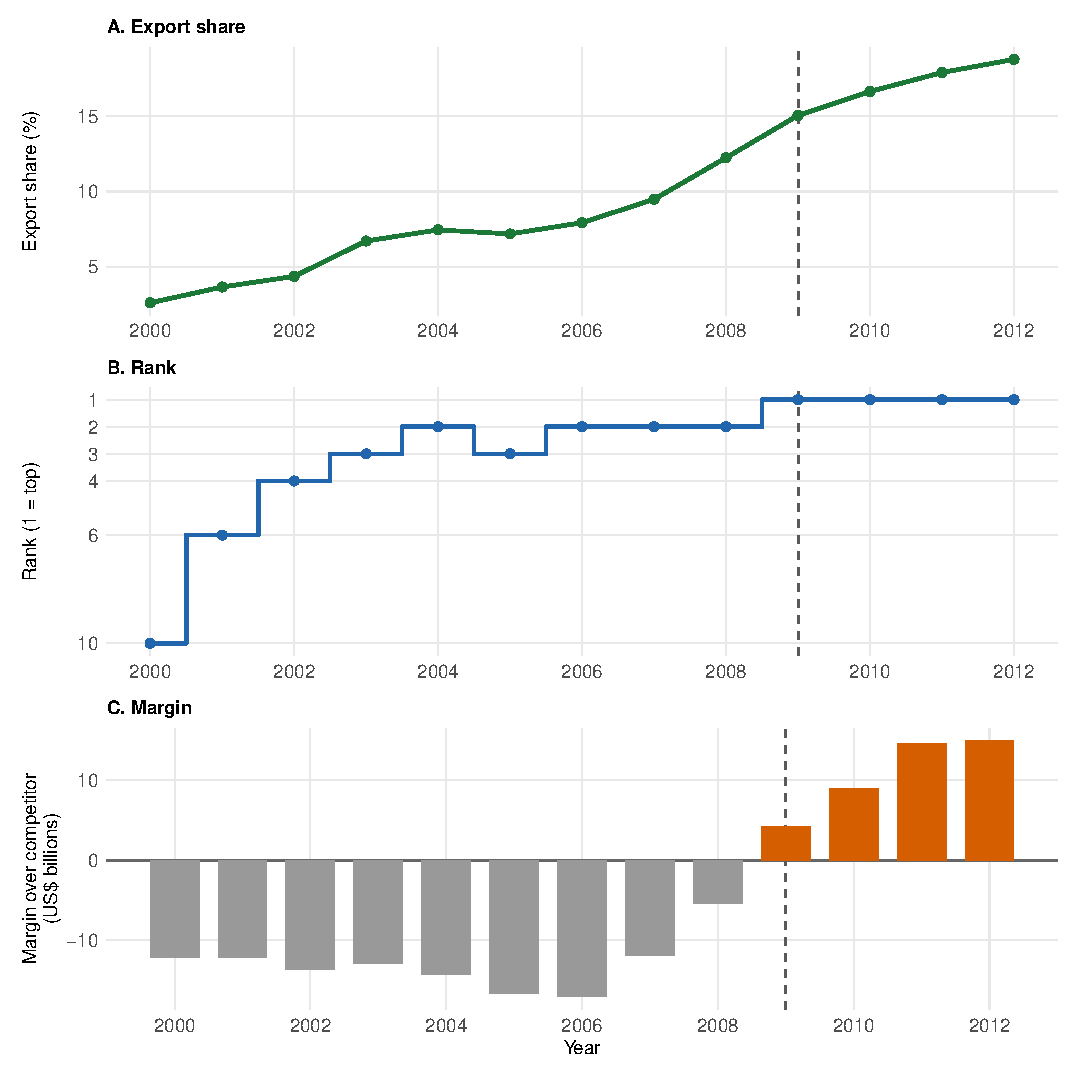
\includegraphics[keepaspectratio,alt={\label{fig:brazil-rank-volume}Brazil rank-versus-volume diagnostic for China's export-destination status. Panels show China's export share, ordinal rank, and signed margin over the relevant competitor. The dashed line marks the 2009 rank reversal. Note: Export share in percent; ordinal rank; export-value margin in current USD billions. Window: 2000-2012 annual Brazil series.}]{figures/brazil-rank-volume-1.pdf}}
\caption{\label{fig:brazil-rank-volume}Brazil rank-versus-volume diagnostic for China's export-destination status. Panels show China's export share, ordinal rank, and signed margin over the relevant competitor. The dashed line marks the 2009 rank reversal. Note: Export share in percent; ordinal rank; export-value margin in current USD billions. Window: 2000-2012 annual Brazil series.}
\end{figure}

Figure \ref{fig:plot-sdid} presents the preferred SDiD fit, estimated without covariates. The estimated reduced-form effect of when China became Brazil's largest export destination is negative: the ATT is -0.273 ideal-point units. Substantively, this is a reduction equivalent to 1.35 standard deviations of Brazil's annual pre-treatment distance to China.

The placebo-based SE is 0.131, and the conventional two-sided normal-approximation p-value is 0.037 with a 95 percent interval {[}-0.529, -0.017{]}. Because the theory predicts convergence, the directionally aligned placebo-in-space rank is 3/96 (p = 0.031); the conservative two-sided absolute rank is 7/96 (p = 0.073). I report both rather than treating either convention as the sole inferential benchmark. Interpreting these finite-sample ranks as p-values requires placebo assignments to be sufficiently comparable to Brazil; the appendix therefore discloses donor exposure and pre-fit sensitivity. Relative to Brazil's pre-treatment mean distance (0.647), the ATT corresponds to a 42.2 percent reduction. Online Resource 1 shows that China's period average changes little around 2009 despite year-to-year volatility, while Brazil shows a more sustained movement toward China.

\begin{figure}[H]
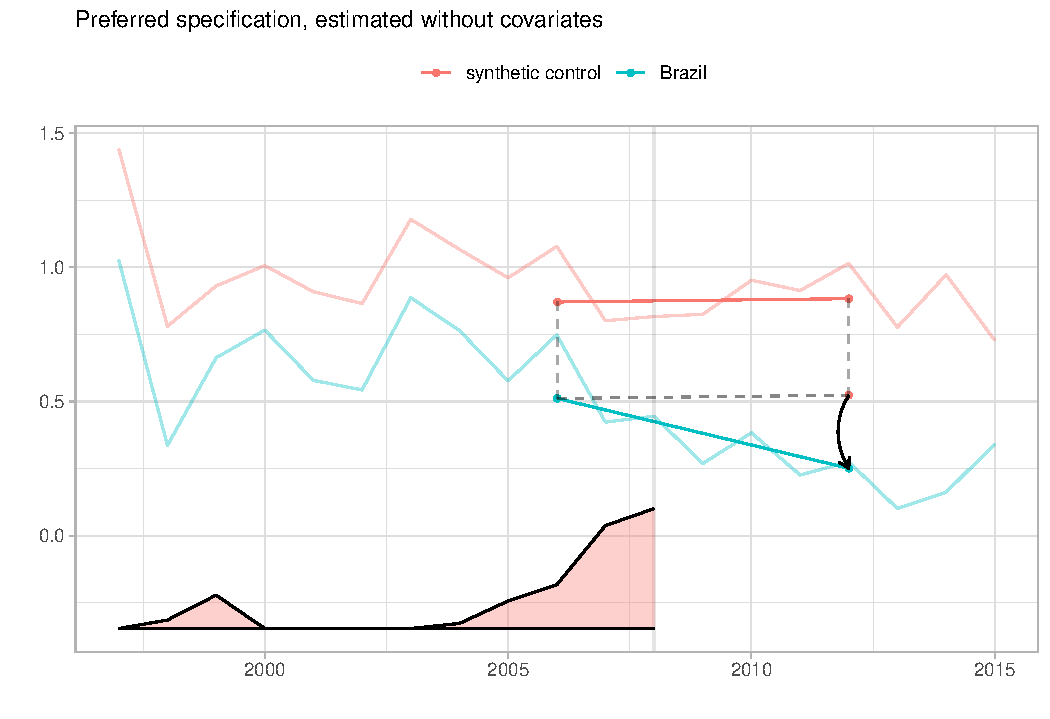
\includegraphics[width=0.95\linewidth]{figures/figure_brazil_sdid_predetermined_core_fit.pdf} \caption{Preferred SDiD fit for Brazil and its synthetic comparison, estimated without covariates. Lower values indicate convergence toward China; the arrow shows the level-adjusted SDiD ATT, equal to the average post-2009 contrast net of the SDiD-weighted pre-treatment contrast; it is not the raw vertical distance between the trajectories. Note: Absolute UNGA ideal-point distance to China. SE: placebo-based SE with 20,000 replications; p-values reported in the text and table. Window: 1997-2015 annual Brazil series.}\label{fig:plot-sdid}
\end{figure}

Figure \ref{fig:plot-placebo-distribution} shows the placebo-in-space distribution behind that inference. Brazil sits in the left tail of the estimates obtained by reassigning treatment to each donor in turn.

\begin{figure}
\centering
\pandocbounded{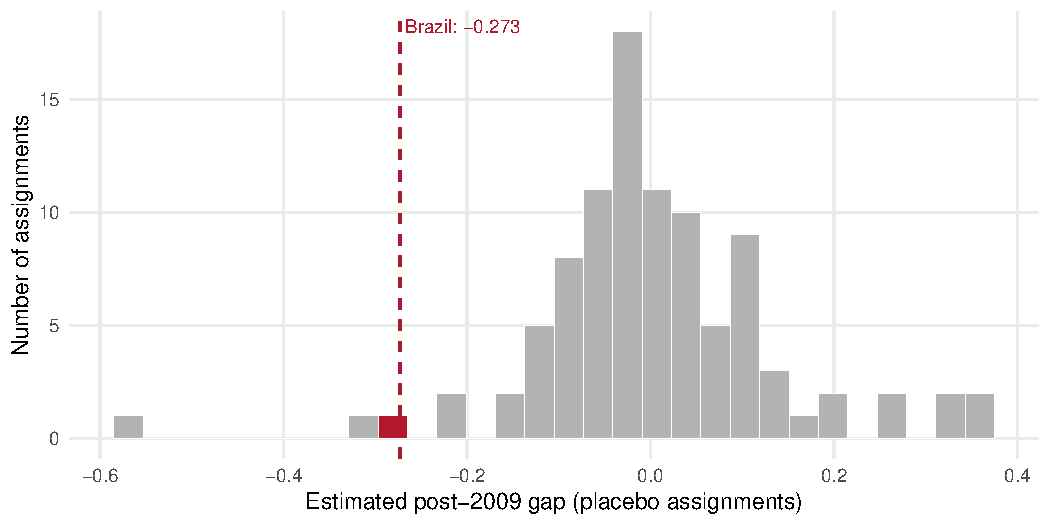
\includegraphics[keepaspectratio,alt={\label{fig:plot-placebo-distribution}Distribution of placebo-in-space estimates across the 95 donor assignments, with Brazil marked. Brazil's estimate is the 3rd most negative of 96 assignments (directional p = 0.031); the two-sided absolute rank is 7/96 (p = 0.073). Negative values indicate convergence toward China. Note: Estimated post-2009 gap in absolute UNGA ideal-point distance to China. Window: 1997-2015 annual SDiD panel.}]{figures/plot-placebo-distribution-1.pdf}}
\caption{\label{fig:plot-placebo-distribution}Distribution of placebo-in-space estimates across the 95 donor assignments, with Brazil marked. Brazil's estimate is the 3rd most negative of 96 assignments (directional p = 0.031); the two-sided absolute rank is 7/96 (p = 0.073). Negative values indicate convergence toward China. Note: Estimated post-2009 gap in absolute UNGA ideal-point distance to China. Window: 1997-2015 annual SDiD panel.}
\end{figure}

Table \ref{tab:brazil-sdid-diagnostic-summary} summarizes the diagnostic package behind the preferred Brazil SDiD estimate. The top five donors are Georgia 3.1\%, Singapore 2.9\%, Chad 2.8\%, Guatemala 2.7\%, Paraguay 2.7\%, and the complete donor pool, along with pre-treatment time weights and sensitivity diagnostics based on donor-deletion and window tests, appears in Online Resource 1.

\clearpage

\begingroup\singlespacing
\renewcommand{\arraystretch}{1.02}
\begin{table}[!h]
\centering
\caption{\label{tab:brazil-sdid-diagnostic-summary}Brazil SDiD diagnostics: fit, placebo inference, and sensitivity. Preferred estimate: -0.273 ideal-point units (1997--2015; treatment begins in 2009).}
\centering
\fontsize{10}{12}\selectfont
\begin{threeparttable}
\begin{tabular}[t]{>{\raggedright\arraybackslash}p{10.6cm}>{\raggedleft\arraybackslash}p{3.7cm}}
\toprule
\textbf{Measure} & \textbf{Result}\\
\midrule
\addlinespace[0.7em]
\multicolumn{2}{l}{\textbf{A. Donor weights: concentration of the comparison group}}\\
\hspace{1em}Number of donors & 95\\
\hspace{1em}Largest donor weight & 3.1\%\\
\hspace{1em}Combined weight of the five largest donors & 14.4\%\\
\addlinespace[0.7em]
\multicolumn{2}{l}{\textbf{B. Pre-treatment fit: prediction error after adjusting levels}}\\
\hspace{1em}Pre-treatment prediction error (RMSPE) & 0.058\\
\hspace{1em}Post-treatment / pre-treatment RMSPE & 5.54\\
\hspace{1em}Brazil's pre-treatment mean distance to China & 0.647\\
\addlinespace[0.7em]
\multicolumn{2}{l}{\textbf{C. Placebo inference: Brazil's rank among all assignments}}\\
\hspace{1em}Directional rank (convergence toward China) & 3/96 (p = 0.031)\\
\hspace{1em}Two-sided rank (absolute effect size) & 7/96 (p = 0.073)\\
\addlinespace[0.7em]
\multicolumn{2}{l}{\textbf{D. Donor sensitivity: exclusions and exposure to China}}\\
\hspace{1em}Largest change when dropping one of the top ten donors & 3.6\%\\
\hspace{1em}Estimate after dropping all ten highest-weight donors & -0.268\\
\hspace{1em}Weight on high-weight donors with China in their top two & 10.2\%\\
\addlinespace[0.7em]
\multicolumn{2}{l}{\textbf{E. Windows and timing: point-estimate diagnostics}}\\
\hspace{1em}Windows with a negative estimate (including preferred) & 7 of 7\\
\hspace{1em}Range of estimates across windows & -0.320 to -0.256\\
\hspace{1em}2004 onset: China rank 2 (post-period: 2004--2008) & -0.109\\
\hspace{1em}2009 onset: China rank 1 (post-period: 2009--2015) & -0.273\\
\bottomrule
\end{tabular}
\begin{tablenotes}
\item \textit{Note: } 
\item SDiD = Synthetic Difference-in-Differences; preferred specification has no covariates. Estimates and root mean squared prediction error (RMSPE) are in absolute UNGA ideal-point distance to China; negative estimates indicate convergence. RMSPE removes the mean pre-treatment gap. Placebo ranks include Brazil and 95 donor assignments; their p-value interpretation requires comparable assignments. In D, changes are relative to the preferred estimate; high-weight donors are the top ten, and exposure means China is a top-two export destination in at least one year during 2009--2015 (share of total donor weight). D--E report point estimates, without recomputed inference. Full donor and time weights and all sensitivity results appear in the appendix. The 2004 and 2009 onset rows use different pre- and post-onset periods and separately fitted counterfactuals; their ordering is suggestive and does not establish a statistically significant difference between effects.
\end{tablenotes}
\end{threeparttable}
\end{table}

\endgroup

Table \ref{tab:outcome-robustness-table} reports the preferred Brazil SDiD estimate alongside four comparisons. Column (1) uses no covariates and is preferred because it avoids conditioning the counterfactual on variables observed after 2009. Column (2) restores the full contemporaneous covariate matrix; column (3) removes institutional variables but retains the other contemporaneous measures; column (4) changes the donor pool to Latin America using the contemporaneous matrix; and column (5) applies the preferred no-covariate specification to that regional pool, which makes it the column comparable with (1). All five estimates are negative, but columns (2)--(4) are sensitivity checks rather than alternative candidates for the main specification.

One may wonder whether a synthetic control built from donors all over the world is a good counterfactual for Brazil. Column (5) re-estimates the preferred specification on a donor pool restricted to Latin American countries. The estimated effect is larger in absolute terms, -0.326 against -0.273 in the global pool, and Brazil is the 2nd most negative of 20 assignments in the directional placebo comparison (p = 0.100). The regional pool is small, which limits what either inference convention can show: with 20 units the rank test cannot fall below 0.050 however extreme Brazil is, and the placebo standard error rises from 0.131 to 0.207, so the normal-approximation interval includes zero. Online Resource 1 reports the regional fit.

\begin{table}[H]
\centering
\caption{\label{tab:outcome-robustness-table}Brazil SDiD estimates across main and robustness specifications.}
\centering
\resizebox{\ifdim\width>\linewidth\linewidth\else\width\fi}{!}{
\fontsize{9}{11}\selectfont
\begin{threeparttable}
\begin{tabular}[t]{lccccc}
\toprule
  & (1) Preferred: no covariates & (2) Current covariates & (3) No institutions & (4) Latin America, covariates & (5) Latin America, none\\
\midrule
ATT & -0.273** & -0.268* & -0.269* & -0.408** & -0.326\\
 & (0.131) & (0.143) & (0.143) & (0.207) & (0.207)\\
\textit{Covariates:} &  &  &  &  & \\
Trade share China &  & $\checkmark$ & $\checkmark$ & $\checkmark$ & \\
Trade share US &  & $\checkmark$ & $\checkmark$ & $\checkmark$ & \\
\addlinespace
Power index (GPI) &  & $\checkmark$ & $\checkmark$ & $\checkmark$ & \\
Power gap to US &  & $\checkmark$ & $\checkmark$ & $\checkmark$ & \\
Per-capita income &  & $\checkmark$ & $\checkmark$ & $\checkmark$ & \\
Exchange rate &  & $\checkmark$ & $\checkmark$ & $\checkmark$ & \\
Geographic distance to US &  & $\checkmark$ & $\checkmark$ & $\checkmark$ & \\
\addlinespace
HoG left ideology &  & $\checkmark$ & $\checkmark$ & $\checkmark$ & \\
Current account (\% GDP) &  & $\checkmark$ & $\checkmark$ & $\checkmark$ & \\
Gov. deficit (\% GDP) &  & $\checkmark$ & $\checkmark$ & $\checkmark$ & \\
Parliamentary system &  & $\checkmark$ &  & $\checkmark$ & \\
Military executive &  & $\checkmark$ &  & $\checkmark$ & \\
\addlinespace
US trade agreement &  & $\checkmark$ &  & $\checkmark$ & \\
Country-years & 1,824 & 1,824 & 1,824 & 380 & 380\\
Donor countries & 95 & 95 & 95 & 19 & 19\\
Donor pool & Global & Global & Global & Latin America & Latin America\\
Time window & 1997-2015 & 1997-2015 & 1997-2015 & 1997-2015 & 1997-2015\\
\bottomrule
\end{tabular}
\begin{tablenotes}
\item \textit{Note: } 
\item The outcome is absolute UNGA ideal-point distance to China; ATT is the estimated average causal effect on Brazil after 2009, so negative values mean convergence. ATTs are reported with three decimals. Placebo-based SEs are in parentheses (20,000 replications for columns (1) and (5), which use the preferred no-covariate specification; 5,000 for comparison columns (2)-(4)). Stars use two-sided normal-approximation p-values based on placebo SEs: * p < 0.10; ** p < 0.05; *** p < 0.01. Checkmarks show included covariate groups. Donor counts exclude Brazil. Column (1) uses no covariates, so its covariate cells are left blank. Columns (2)-(4) use contemporaneous covariates and are comparisons. Column (5) applies the preferred no-covariate specification to the Latin American donor pool, so it is the column comparable with (1); its directional placebo rank is 2/20 (p = 0.100), against a floor of 0.050 imposed by the size of the regional pool. For column (1), the directional rank is 3/96 (p = 0.031) and the bilateral absolute rank is 7/96 (p = 0.073).
\end{tablenotes}
\end{threeparttable}}
\end{table}

The rank interpretation requires more than showing that trade with China was increasing. Brazil's exports to China grew before 2009, including years in which China rose in the export hierarchy but did not become number one. Table \ref{tab:table-placebo} therefore reports outcome-path timing falsifications without covariates: using no covariates prevents variables measured after the early pseudo-onsets from entering those comparisons. The 2003, 2004, and 2005 estimates are smaller in absolute value than the 2009 rank-one estimate; 2004 is especially useful because China first reaches rank 2 but is still not Brazil's largest export destination. The 2012 row probes a later break after China had already become the top destination. Each row refits the SDiD counterfactual over a different pre- or post-onset window. The early estimates average 2003--2008, 2004--2008, and 2005--2008, compared with 2009--2015 for the preferred estimate and 2012--2016 for the later break. Their ordering is suggestive timing evidence, not a comparison of a common estimand or a test that the effects differ. No uncertainty for differences between rows is reported, and the 2012 fit uses already-treated years in its nominal pre-period.

The same timing logic addresses the main Brazilian political confounder. President Lula da Silva took office in 2003 and pursued a more explicit South-South foreign-policy agenda, a shift emphasized in work on Brazilian autonomy, presidential foreign policy, and international engagement \citep{neto2011, mouron_urdinez2014, neto_malamud2015, rodrigues2019measuring, schenoniMythsMultipolaritySources2022}. The 2003 and 2005 pseudo-onsets yield smaller point estimates in absolute value, providing suggestive evidence against an immediate large break. Because these estimates cover different periods and refit the counterfactual, they do not establish that the early and 2009 effects differ or exclude a gradual or delayed Lula-era shift. The cross-country panel also estimates the rank-threshold pattern across countries with different political systems and leadership profiles, which reduces the concern that the Brazil estimate is only a Lula-period artifact.

The main rival explanation for the proposed effect of a discrete status change is that Brazil's estimated convergence simply reflects a continuous increase in its export dependence on China. Under this account, UNGA alignment should respond smoothly to the degree of trade exposure to China. The pattern shown in Figure \ref{fig:brazil-rank-volume} is compatible with this possibility: Brazil's export exposure increased well before 2009, raising the concern that nothing distinctive occurred at the rank-one threshold and that the estimated effect instead reflects Brazil's growing commercial ties with China.

To assess this possibility, I relate each donor country's placebo-in-space pseudo-ATT to the change in its export share directed to China. By construction, the donor pool excludes countries in which China became the largest goods-export destination during the 1997--2015 estimation window. These countries therefore provide variation in trade exposure below the rank-one threshold. If continuous exposure drives alignment, donors experiencing larger increases in exposure should exhibit more negative pseudo-ATTs -- that is, greater convergence toward China. A flat or positive relationship would instead weaken this rival explanation, although it would not by itself establish that status is the operative mechanism.

Figure \ref{fig:rival-hypothesis} provides little support for the continuous-exposure account. Panel A measures exposure using goods trade, matching the sectoral definition used to assign treatment, while Panel B uses all-sector trade, including both goods and services. The relationship is essentially flat under both measures. The OLS slopes are 0.0002 and 0.0007 per percentage point, respectively, while the corresponding Spearman correlations are 0.034 and 0.037. Under either measure, Brazil's ATT is also more negative than those of 23 of the 24 donors in the highest quartile of exposure growth. These patterns do not rule out a role for continuous export dependence, nor do they identify a discontinuity at the rank threshold itself, but they make it less plausible that Brazil's result is driven simply by rising trade exposure to China.

\begin{figure}[!htbp]
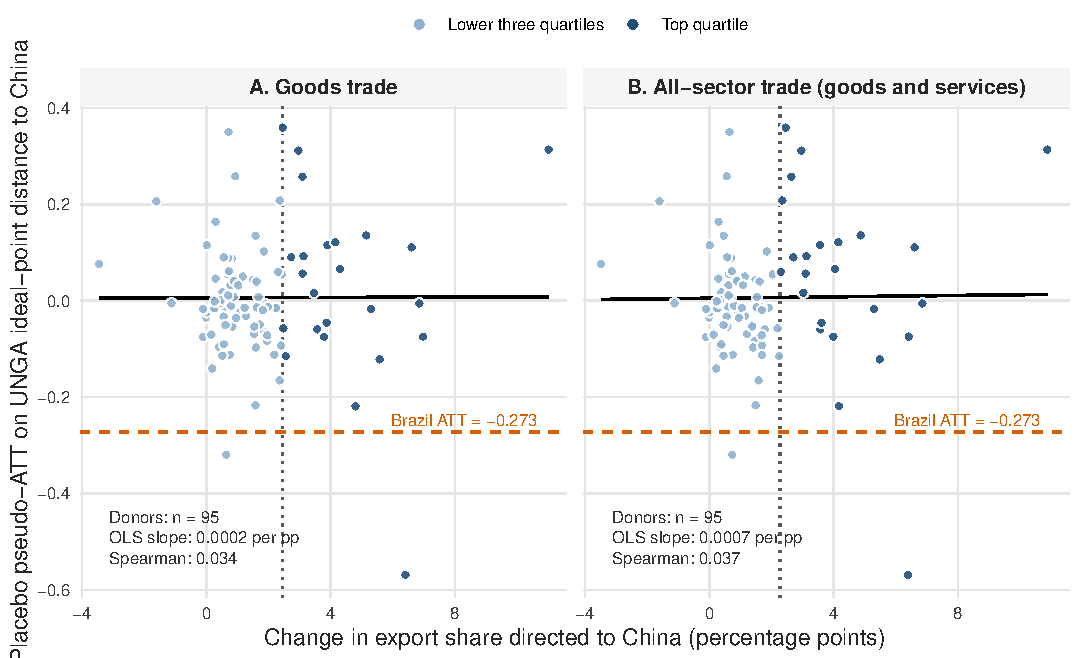
\includegraphics[width=1\linewidth]{figures/figure_brazil_sdid_dose_response_panel.pdf} \caption{Trade-exposure dose and placebo-in-space pseudo-ATTs among 95 donor countries. Each donor is assigned the same 2009 pseudo-treatment, and dose is the difference between its mean annual export share directed to China in 2009--2015 and 1997--2008. Panel A measures goods trade; Panel B measures all-sector trade, including goods and services. Negative pseudo-ATTs indicate convergence toward China. Dark points identify donors in the top quartile of dose, vertical dotted lines mark the corresponding cutoffs, and black lines are descriptive OLS fits. The orange dashed horizontal line marks Brazil's ATT of -0.273; Brazil has no dose coordinate and therefore does not enter either fit. No donor had China as its largest goods-export destination during 1997--2015, so the figure shows only the dose gradient below the rank-one threshold and does not identify a discontinuity at that threshold. Donor pseudo-ATTs are estimated from overlapping pools, so no standard error is reported for either slope.}\label{fig:rival-hypothesis}
\end{figure}

A remaining concern is that 2009 bundled the Brazilian rank reversal with other contemporaneous shocks, including the global financial crisis, the BRICS/G20 moment, and the commodity cycle. Table \ref{tab:china-demand-sdid-diagnostics} uses measures built from external goods exports only to address this critique. The exposure baselines are country means over 2004--2008: primary goods as a share of external goods exports, its Agriculture and Mining and Energy components, and China as a share of external goods exports. In the table, \texttt{x\ 2008-\/-2009} means that the fixed 2004--2008 exposure is multiplied by an indicator for 2008 and 2009 and then standardized over the stored 1997--2016 input panel before restriction to the 1997--2015 estimation window. The price diagnostic instead weights World Bank Pink Sheet log-price changes relative to 2007 by the country's 2004--2008 Agriculture, Energy, and Metals and Minerals export shares, activates that index in 2008--2009, and standardizes it over the same stored 1997--2016 input panel before the 1997--2015 estimation-window restriction. Only these time-varying interactions enter the four diagnostic specifications: exposure levels are time-invariant and absorbed by unit effects, while the common 2008--2009 indicator is absorbed by time effects.

Brazil's 2004--2008 primary-goods share is 29.04 percent, composed of 11.25 percent Agriculture and 17.79 percent Mining and Energy. The preferred ATT is -0.273; adding primary composition and its 2008--2009 interaction yields -0.285. Composition, decomposition, global-price, and prior-China-exposure specifications remain in a narrow negative range. The 2008--2009 interactions are robustness or mechanism diagnostics, not alternative total-effect estimates, because 2009 is the first treated year and the interaction may absorb part of the mechanism. Stability across these measures does not isolate the rank cue experimentally from every 2009 political shock, but it reduces the narrower concern that the preferred estimate is an artifact of post-treatment controls or omitted pre-2009 commodity composition.

The cross-country panel below is a broader scope check, not the main answer to the Brazil-specific demand-shock critique. Brazil is included in the goods-only cross-country sample, but the panel aligns countries by their own China-top goods-export entry years. A Brazil-specific 2009 confounder cannot mechanically generate an average event-time effect across countries treated in different calendar years. For such an explanation to account for both the Brazil estimate and the cross-country result, the omitted force would need to coincide with durable China-top entry across countries, affect UNGA distance to China in the same direction, and remain outside the latent factors captured by the interactive fixed-effects specification. It would also need to be strongly enough associated with both treatment timing and the outcome to overturn estimates that are stable across the donor-pool checks and the cross-country duration and risk-set checks, alongside the suggestive Brazil timing diagnostics.

\begin{table}[H]
\centering
\caption{\label{tab:table-placebo}Brazil SDiD rank-versus-volume timing diagnostics without covariates.}
\centering
\resizebox{\ifdim\width>\linewidth\linewidth\else\width\fi}{!}{
\fontsize{8}{10}\selectfont
\begin{threeparttable}
\begin{tabular}[t]{clccccl}
\toprule
Timing year & Test role & China rank & Export share (\%) & Margin (USD bn) & ATT & Inference\\
\midrule
2003 & Growth/lower-rank promotion & 3 & 6.7 & -12.9 & -0.064 & Point estimate only; no covariates\\
2004 & China rank-2 threshold & 2 & 7.4 & -14.2 & -0.109 & Point estimate only; no covariates\\
2005 & Rapid growth without rank 1 & 3 & 7.2 & -16.7 & -0.099 & Point estimate only; no covariates\\
2009 & Actual rank-1 reversal & 1 & 15.1 & 4.1 & -0.273 & Point estimate only; no covariates\\
2012 & Later-break falsification & 1 & 18.8 & 14.9 & -0.100 & Point estimate only; no covariates\\
\bottomrule
\end{tabular}
\begin{tablenotes}
\item \textit{Note: } 
\item Outcome is absolute UNGA ideal-point distance to China; ATT denotes the SDiD estimate for Brazil after each nominal onset; negative values indicate convergence; export margins are current USD billions. Window: all windows begin in 1997. Post-onset periods are 2003-2008, 2004-2008, 2005-2008, 2009-2015, and 2012-2016 (6, 5, 4, 7, and 5 years). All rows use Brazil and the same 95 donors, without covariates, but refit unit and time weights for each window and onset. These are suggestive diagnostics with different estimands, not tests of differences between effects; no uncertainty for the cross-row contrasts is reported. The 2012 nominal pre-period includes already-treated years. The preferred 2009 estimate and its inference are reported separately in the main specification.
\end{tablenotes}
\end{threeparttable}}
\end{table}

\begin{table}[H]
\centering
\caption{\label{tab:china-demand-sdid-diagnostics}Brazil SDiD estimates under corrected predetermined commodity and China-demand diagnostics.}
\centering
\fontsize{9}{11}\selectfont
\begin{threeparttable}
\begin{tabular}[t]{lcccc}
\toprule
Specification & ATT & Placebo SE & Normal p & Rank p (dir./bilat.)\\
\midrule
Current covariates & -0.268 & 0.143 & 0.061 & Not computed\\
Preferred: no covariates & -0.273 & 0.131 & 0.037 & 0.031 / 0.073\\
Primary share x 2008-2009 & -0.285 & 0.129 & 0.027 & 0.031 / 0.073\\
Agriculture/mining x 2008-2009 & -0.284 & 0.128 & 0.026 & Not computed\\
Price exposure x 2008-2009 & -0.277 & 0.130 & 0.034 & Not computed\\
\addlinespace
Prior China share x 2008-2009 & -0.284 & 0.130 & 0.029 & Not computed\\
\bottomrule
\end{tabular}
\begin{tablenotes}
\item \textit{Note: } 
\item Outcome is absolute UNGA ideal-point distance to China; ATT is the estimated average causal effect on Brazil after 2009, so negative values mean convergence. SE: synthdid placebo SE with 20,000 replications for the preferred row and 5,000 with a common seed for comparison rows. Window: 1997-2015 annual SDiD panel. All rows keep the binary 2009 onset. The preferred row uses no covariates; other rows are diagnostics, and the 2008--2009 interactions include the first treated year. Rank inference was computed only for the preferred and primary-share interaction rows; 'Not computed' does not denote a failed test.
\end{tablenotes}
\end{threeparttable}
\end{table}

\subsection{Issue-Area Evidence: Where Did Convergence Occur?}\label{issue-area-evidence-where-did-convergence-occur}

The aggregate ideal-point estimate raises a substantive question: in what kinds of votes did Brazil move closer to China? Resolution-level diagnostics suggest that the post-2009 convergence was selective rather than uniform. Figure \ref{fig:plot-brazil-china-unvotes-issue-year} disaggregates the convergence rate by year and substantive issue family. In several issue areas Brazil and China already voted together at high rates before treatment, leaving little room for additional convergence. The more informative domain is human rights, where pre-treatment agreement was lower and where movement toward China carried greater reputational costs for Brazil, given the domestic and international implications of Brazil's human-rights foreign policy \citep{milani2015humanrights}.

\begin{figure}
\centering
\pandocbounded{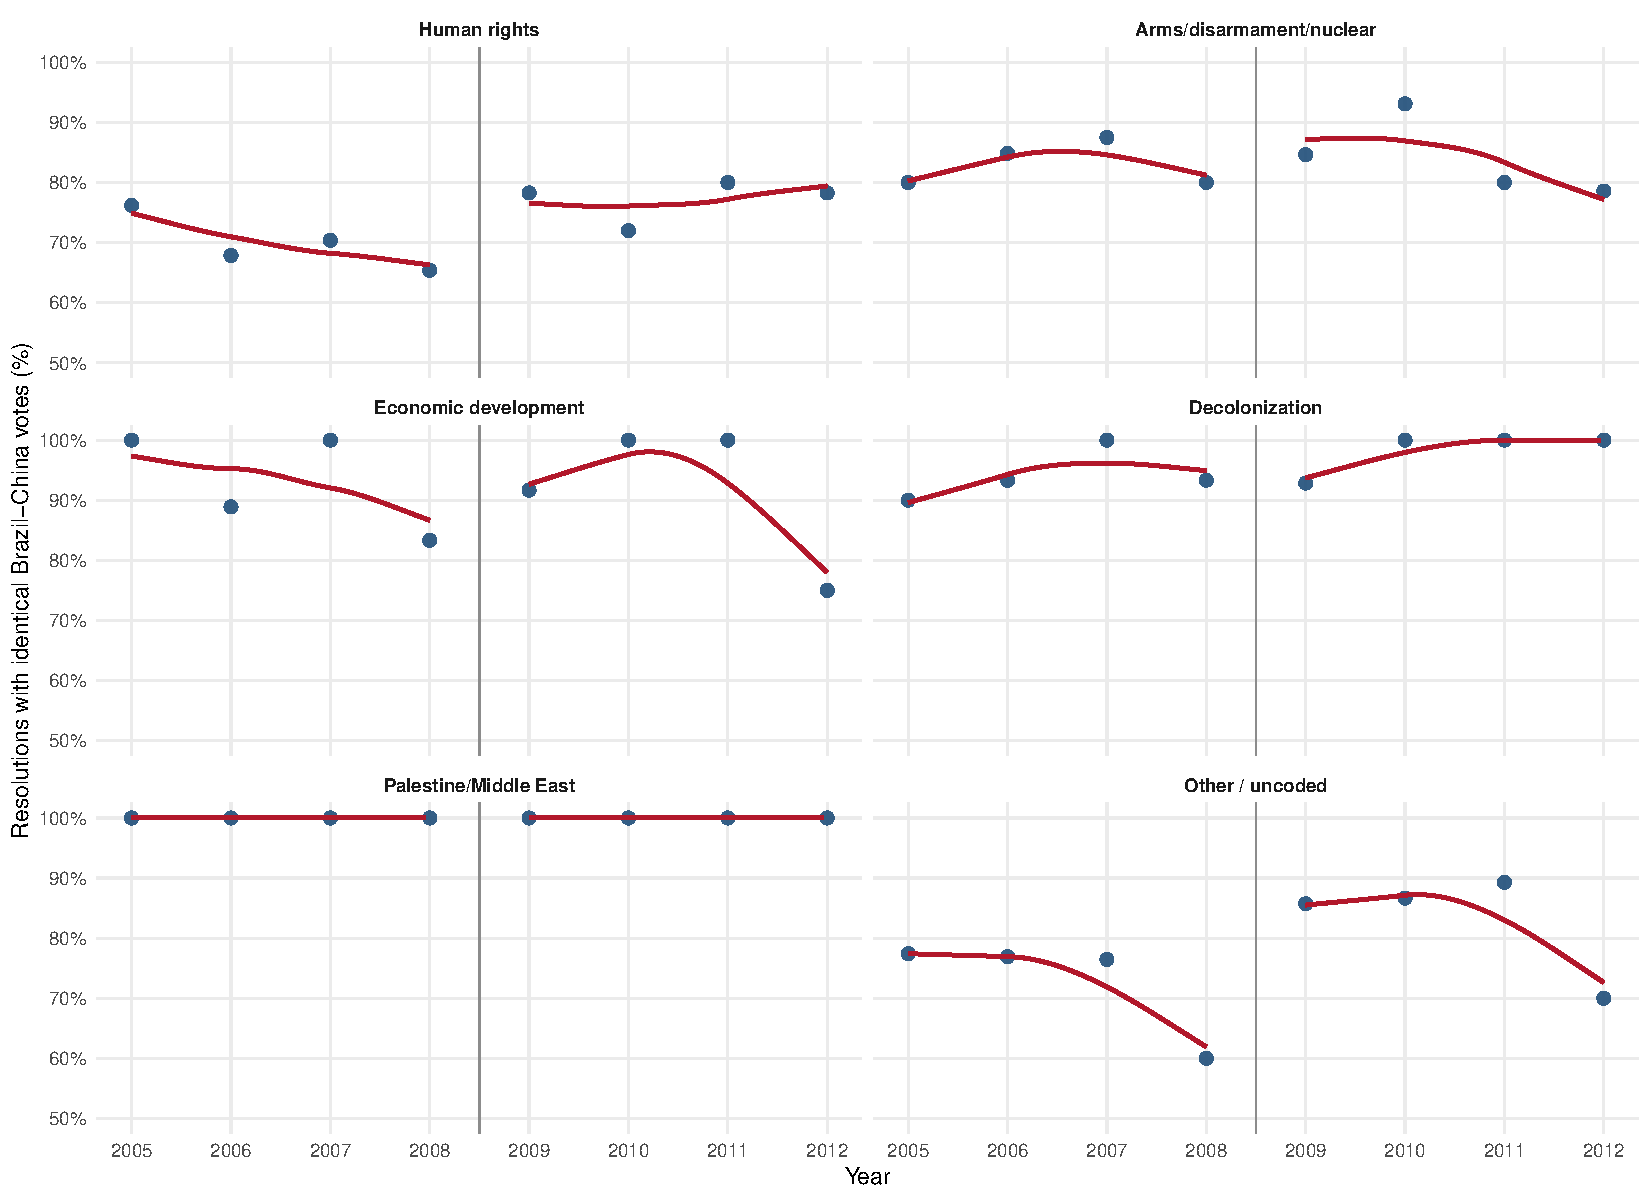
\includegraphics[keepaspectratio,alt={\label{fig:plot-brazil-china-unvotes-issue-year}Brazil-China identical UNGA votes by issue area, 2005-2012. Points report annual shares; the vertical line marks 2009. The clearest pattern expected by the mechanism is selective convergence in human rights. Note: Percentage of roll-call resolutions with identical Brazil-China votes. Window: 2005-2012 annual series; multi-coded resolutions enter each issue family.}]{figures/plot-brazil-china-unvotes-issue-year-1.pdf}}
\caption{\label{fig:plot-brazil-china-unvotes-issue-year}Brazil-China identical UNGA votes by issue area, 2005-2012. Points report annual shares; the vertical line marks 2009. The clearest pattern expected by the mechanism is selective convergence in human rights. Note: Percentage of roll-call resolutions with identical Brazil-China votes. Window: 2005-2012 annual series; multi-coded resolutions enter each issue family.}
\end{figure}

In that domain, Brazil-China identical voting increased by 7.5 percentage points after 2009. This pattern is consistent with the proposed mechanism because it locates the clearest movement in a visible multilateral arena where Brazil had previously maintained more distance. It does not, however, show that the trade-rank cue itself caused the selective shift or that policymakers relied on it in particular decisions.

The strongest support comes from human-rights resolutions in which China and the United States diverged, where Brazil moves closer to China relative to comparable donor countries after 2009.

This descriptive increase does not by itself establish China-specific alignment, because annual issue-area shares can reflect agenda composition and do not compare Brazil with donor countries. To address such issues, I ran regressions with country and resolution fixed effects, restricted to human-rights votes where China and the United States cast different votes.

The results show that Brazil moves closer to China after 2009 relative to the donor pool. The Brazil-by-post-2009 coefficient is -0.357 for distance to China minus distance to the United States (model-based SE = 0.021), and -0.414 when the sample is restricted to strong yes/no China-US disagreements (model-based SE = 0.023). The corresponding non-human-rights estimate is smaller (-0.131, model-based SE = 0.012). These are not causal estimates, given the usual selection and omitted-variable concerns.

However, restricting attention to a single issue domain opens a design that ideal points computed over all votes cannot support: a triple difference. Ideal points compress every resolution in a session into one score, leaving no contrast between issue domains to exploit, whereas vote-level data preserve it. Thus, I can not only compare the difference between Brazil and other untreated countries before and after (traditional DiD), but also include a third difference: across domains within the same country and year, comparing Brazil with the donor pool, before and after 2009, in human-rights votes relative to every other vote. Identification here asks for more than parallel trends between treated and control units: whatever bias a non-parallel trend introduces must be the same in the two issue domains, so that it cancels in the third difference \citep{olden_moen2022}. Online Resource 1 displays the pre- and post-2009 Brazil-donor gaps in both domains; this descriptive comparison does not establish the identifying restriction.

Let \(B_i\) identify Brazil, \(P_r\) indicate 2009--2012, and \(H_r\) identify a human-rights resolution. The vote-level specification is
\[
Y_{ir}=\alpha_i+\lambda_r+\beta(B_iP_r)+\gamma(B_iH_r)+\delta(B_iP_rH_r)+\varepsilon_{ir}.
\]
Country and resolution fixed effects absorb the remaining lower-order terms. The Brazil-by-domain interaction allows Brazil's pre-existing gap relative to donors to differ between human-rights and other resolutions. The coefficient \(\delta\) measures the additional post-2009 human-rights shift. The sample contains 55,190 observed votes by 95 countries on 612 China-US divergent resolutions in 2005--2012. Votes are scored \(-1\) for no, \(0\) for abstain, and \(1\) for yes. The outcome is \(Y_{ir}=|s_{ir}-s_{Cr}|-|s_{ir}-s_{Ur}|\), where \(s_{Cr}\) and \(s_{Ur}\) are China's and the United States' scores; negative values indicate a vote closer to China. Country-resolution pairs without a recorded yes, no, or abstain vote -- whether because of absence, nonparticipation, or another reason -- do not enter the observed-vote sample. A resolution enters the China-U.S. divergent sample only when both China and the United States have recorded votes and their scores differ. Any human-rights tag places a resolution in the human-rights group; all remaining resolutions form the non-human-rights group. Each observed country-resolution vote receives equal weight. The specification does not absorb a separate domain intercept for each donor country; interpretation also requires changes in donor vote availability not to generate the differential shift across domains.

The DDD estimate is -0.222 for distance to China minus distance to the United States (country-clustered model-based SE = 0.014). Its negative sign indicates a larger shift toward China in human-rights votes. With Brazil as the single treated country, I also reassign the treated-country role to each country, rebuilding all three interactions and retaining the same sample and fixed effects. In this DDD-specific distribution, Brazil ranks 9 of 95 in the predicted direction (inclusive directional tail share = 0.095; strict donor-only share = 0.085; two-sided absolute share = 0.126). These are descriptive reassignment benchmarks; interpreting them as randomization inference requires exchangeability of country assignment.

The separate human-rights-only DiD estimate of -0.357 ranks 6 of 95 in its own country-placebo distribution (inclusive directional share = 0.063; strict donor-only share = 0.053). This benchmark evaluates the within-domain post-2009 contrast, whereas the DDD benchmark evaluates the additional shift across domains.

\begin{table}[H]
\centering
\caption{\label{tab:issue-area-prepost-table}Brazil-China identical UNGA votes by issue area, before and after 2009.}
\centering
\resizebox{\ifdim\width>\linewidth\linewidth\else\width\fi}{!}{
\fontsize{8}{10}\selectfont
\begin{threeparttable}
\begin{tabular}[t]{lrrrl}
\toprule
Issue area & Pre-2009 identical vote share & Post-2009 identical vote share & Change & Interpretation\\
\midrule
Human rights & 69.6 & 77.1 & 7.5 & Politically costly convergence; mechanism-informative\\
Arms/disarmament/nuclear & 83.0 & 84.3 & 1.2 & Diagnostic evidence\\
Economic development & 92.9 & 90.0 & -2.9 & Diagnostic evidence\\
Decolonization & 94.1 & 98.1 & 4.0 & Diagnostic evidence\\
Palestine/Middle East & 100.0 & 100.0 & 0.0 & High baseline agreement; limited room to move\\
\addlinespace
Other / uncoded & 73.4 & 83.1 & 9.7 & Heterogeneous residual category\\
\bottomrule
\end{tabular}
\begin{tablenotes}
\item \textit{Note: } 
\item Percentage of roll-call resolutions with identical Brazil-China votes. Window: 2005-2008 versus 2009-2012; multi-coded resolutions enter each issue family. Rows are label-specific diagnostics, not a mutually exclusive decomposition of the aggregate convergence pattern.
\end{tablenotes}
\end{threeparttable}}
\end{table}

The DDD estimate indicates a larger human-rights shift than the analogous non-human-rights shift. Its country-placebo distribution provides moderate evidence for that additional shift and counsels against language implying that Brazil is unique. The Brazil evidence therefore supports a cautious claim of selective UNGA adjustment toward China in politically visible domains, rather than a claim that Table \ref{tab:issue-area-prepost-table} alone proves selective convergence.

\section{Brazilian Media Salience}\label{brazilian-media-salience}

To assess whether trade-topic salience increased around the rank reversal, I examine coverage of China in Folha de S.Paulo, Brazil's widest-circulation newspaper \citep{folha2016}, from 2000 to 2014. Salience matters because the rank-threshold argument requires the top-rank cue to become politically usable. A change in export hierarchy can shape elite and public attention when it appears in a prominent national newspaper as a simple signal of China's commercial importance, consistent with work on media, agenda setting, and foreign policy \citep{soroka2003, baum_potter2008, walgraveContingencyMassMedias2006}.

Headlines are the appropriate unit for this trade-topic diagnostic because they are tractable in large archives and operate as attention-directing cues \citep{zhang_yu2024_chinese_dream}. The relevant question is whether Folha increasingly foregrounded China as a trade relationship after the rank reversal. Headlines are the most visible textual cue in the archive and the part of coverage most likely to be scanned by broad audiences. Full article texts would be useful for a different exercise -- for example, measuring tone or detailed argumentation -- but the salience claim here is about which China-related themes were made visible at the headline level. This diagnostic does not measure the frequency of explicit rank labels.

The preserved retrieval code specifies a Folha site search for \texttt{china}, orders the results from oldest to newest, extracts the displayed title and date, retains one record per exact title, and then keeps titles containing \texttt{China}, \texttt{chinês}, or \texttt{chinesa}. The classified headline file is frozen as an analysis input rather than regenerated during manuscript rendering. The archive does not contain the raw page responses or contemporaneous page-level logs needed to certify the historical search as exhaustive, and the boundary years 2000 and 2014 do not have complete annual coverage.

I therefore classify China-related headlines into substantive categories and then collapse them into four analytically relevant groups: China-Brazil trade, China's domestic economy, diplomacy and bilateral relations, and non-economic coverage. The classification uses a fixed label set with examples, and the appendix reports the exact prompt and validation procedure. Figure \ref{fig:plot-media-counterfactual} compares 2000--2008 with 2009--2014 and shows a substantial increase in China-Brazil trade coverage, from an average of 47 to 73 headlines per year (about 55 percent), alongside a larger increase in coverage of the Chinese economy, from 147 to 311 headlines per year (about 111 percent). Together, these patterns are consistent with increased media attention to China's economic importance for Brazil, as the proposed mechanism predicts. The figure supports the trade-topic-salience step, but it does not by itself establish the public availability of an explicit rank cue. The separate contemporary sources below provide evidence about rank language.

\begin{figure}
\centering
\pandocbounded{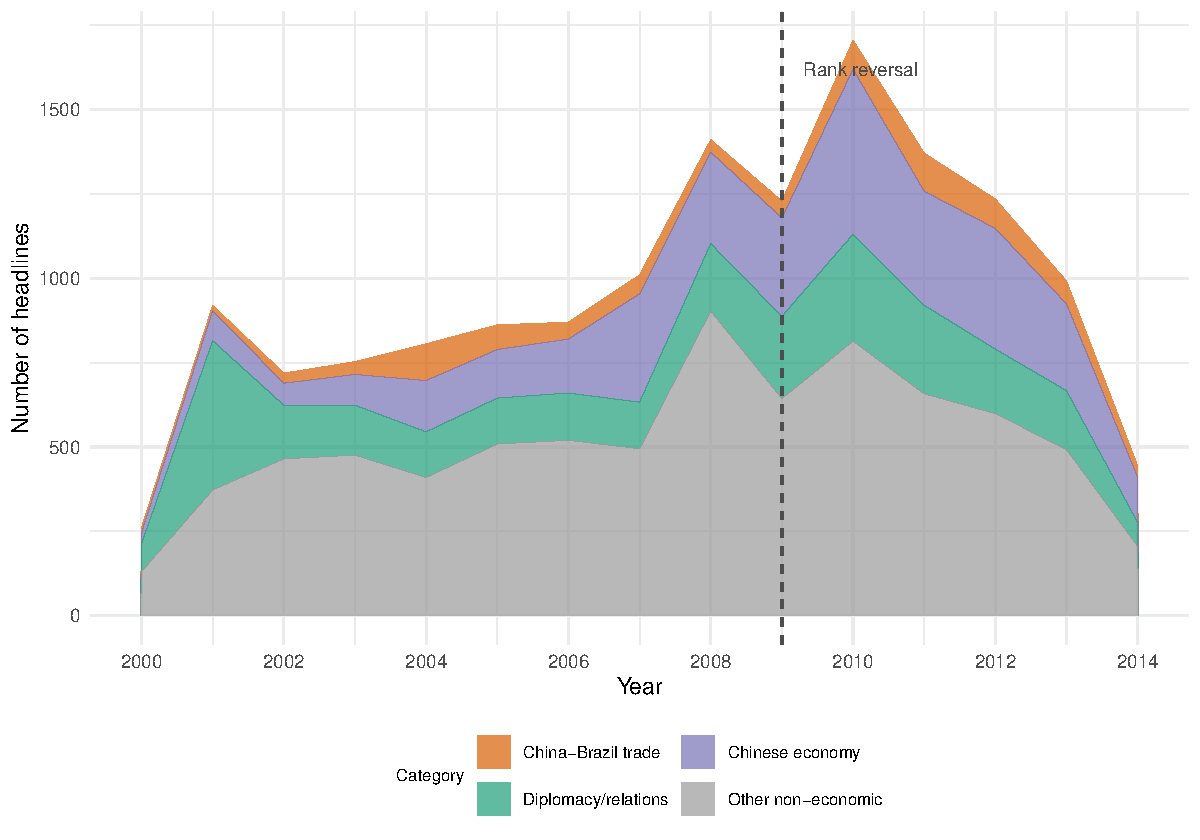
\includegraphics[keepaspectratio,alt={\label{fig:plot-media-counterfactual}Brazilian media salience: disaggregated China headlines in Folha de S.Paulo by category. From 2000--2008 to 2009--2014, China-Brazil trade coverage increases substantially and coverage of the Chinese economy increases even more; together, the changes are consistent with heightened attention to China's economic importance for Brazil. Note: Headlines per category per year. Window: 2000-2014 annual series.}]{figures/plot-media-counterfactual-1.pdf}}
\caption{\label{fig:plot-media-counterfactual}Brazilian media salience: disaggregated China headlines in Folha de S.Paulo by category. From 2000--2008 to 2009--2014, China-Brazil trade coverage increases substantially and coverage of the Chinese economy increases even more; together, the changes are consistent with heightened attention to China's economic importance for Brazil. Note: Headlines per category per year. Window: 2000-2014 annual series.}
\end{figure}

\clearpage

The evidence distinguishes public availability from official uptake. The status cue became publicly available during the 2009 treatment year, before the full-year trade table was finalized. In early May, contemporary coverage of January--April trade statistics reported a historic shift in Brazil's trade hierarchy: China had become Brazil's largest trading partner and had purchased US\$5.627 billion in Brazilian exports, compared with US\$4.925 billion purchased by the United States \citep{agencia_brasil2009_china_supera}. This real-time visibility matters for the mechanism. The empirical design codes treatment annually because the outcome and comparative trade data are annual, but officials, journalists, and firms encountered the rank cue through contemporaneous monthly and year-to-date statistics. Lula's May 2009 Beijing visit then provides evidence of official uptake during the treatment year: the new rank was already available as a public category around which diplomatic priorities could be narrated. Brazilian officials subsequently invoked China's new position in Brazil's trade hierarchy when explaining diplomatic prioritization, bilateral upgrading, and institutional follow-up.

In a written interview on the eve of his May 2009 visit to Beijing, President Lula described China as Brazil's leading trading partner and framed the trip as an effort to consolidate cooperation across commerce, technology, and global economic governance \citep[323]{mre_funag_resenha104_2009}. In Beijing three days later, Lula repeated the rank claim in speeches organized around the Brazil-China Strategic Partnership, trade diversification, investment, presidential diplomacy, and the preparation of the 2010--2014 Joint Action Plan \citep[115, 121--122]{mre_funag_resenha104_2009}. The cue then persisted in Itamaraty language. When announcing Hu Jintao's 2010 state visit and the signature of the Joint Action Plan, the Ministry of Foreign Affairs again invoked China's 2009 rise to the top of Brazil's trade hierarchy \citep[356]{mre_funag_resenha106_2010}. Dilma Rousseff and Hu Jintao's 2011 joint communiqué likewise noted that China had become Brazil's principal trading partner in 2009 and embedded that status in an agenda of intensified dialogue over trade, investment, diversification, and implementation of the Joint Action Plan \citep[160--161]{mre_funag_resenha108_2011}. Later that year, Foreign Minister Antonio Patriota made the institutional link explicit: in discussing China, he announced a dedicated Itamaraty task force to monitor economic-commercial relations with Brazil's principal trading partner and to propose ways to move the relationship beyond complementarity, toward diversification and higher value-added trade \citep[47]{mre_funag_resenha109_2011}.

These statements show official uptake of the 2009 status cue. Their co-occurrence with diplomatic prioritization and institutional attention is consistent with justificatory use, but it does not demonstrate that the cue caused those initiatives or particular UNGA decisions. The evidence therefore supports the availability and uptake steps directly and treats justificatory use as an inference compatible with the public mechanism implied by the theory: once China was officially recognized as central in Brazil's economic hierarchy, selective diplomatic accommodation could be presented as pragmatic recognition of national economic interests rather than as ideological concession or opportunistic bandwagoning.

\section{Cross-Country Evidence Beyond Brazil}\label{cross-country-evidence-beyond-brazil}

The cross-country analysis serves two purposes. First, it examines whether a first position as a goods export destination is followed by movement toward China beyond the Brazilian case. Second, it is an additional robustness check against explanations tied specifically to Brazil's 2009 calendar year, such as the global financial crisis, the BRICS/G20 moment, or the commodity cycle.

However, operationalizing the analysis with multiple countries poses several difficulties. As the formal model shows, the public cue should increase the probability of a policy shift, all else equal.\footnote{Strictly speaking, the model is deterministic. Here, however, I treat the timing of treatment as stochastic, which allows me to speak of an increase in probability.} Thus, with the assistance of artificial intelligence, I searched press sources for all potentially treated countries in which a public cue could have occurred. I found high-quality data only for Australia, Chile, Uruguay, Gabon, and Qatar. However, since absence of evidence is not evidence of absence, I cannot say that no public cue occurred in the other countries. Thus, because public salience is not measured directly outside Brazil, the panel does not by itself validate the top trade rank position as a proxy for public status change or extend the public cue mechanism to the larger sample.

Another difficulty is that the treatment is the public cue, but the model does not distinguish which trade statistic drives it. For each country, the cue may occur when China becomes the leading destination for merchandise exports alone; in countries where services matter more, it may instead arise from goods and services combined, or even services alone; and in other cases, it may be total trade flows (exports plus imports). Thus, for each country, it is unclear which statistic is relevant for identifying a potential treatment. The Australian case is illustrative. The Australian Financial Review (AFR) headlines said ``China hits the spot as trading partner'', referring to imports plus exports and mentioning in the text that 2009 was the third year it was in that leading position. To complicate matters further, AFR uses the fiscal year 2006-2007, not the calendar year. Should I code the beginning of treatment in 2010 (when China became the top export destination), 2007 (when I found the public cue evidence), or perhaps 2008 (because the fiscal year ended mid-2007)? Finally, if a country is already very close to China before treatment---as is the case of Gabon; see Online Resource 1---there are no gains from shifting its foreign-policy stance.

To address these problems, I estimated a separate SDiD model for each of the countries for which I have data on the public cue and in which there was room for foreign-policy adjustment toward China: Chile, Uruguay, and Australia. I excluded Gabon, which was already very close to China before treatment, and Qatar, whose treatment occurred only in 2021, leaving too little time for the effect to emerge. For Australia, I use 2007 as the theoretically preferred public-cue date and retain 2010, when China became the top goods-export destination, as a robustness timing. The corresponding estimand is the ATT on absolute UNGA ideal-point distance to China.

The case-specific estimates are mixed (see Online Resource 1). Chile and Uruguay have negative estimates, in the direction of convergence, but both are imprecise. The Australian estimates for 2007 and 2010 are positive, in the direction of greater distance from China, and are also imprecise. All four 95 percent intervals include zero. For the theoretically preferred 2007 public-cue timing, the ATT is 0.128 ideal-point units (placebo SE = 0.161; two-sided normal-approximation p = 0.424; 95 percent CI: {[}-0.187, 0.444{]}). The p-value and interval use a normal approximation based on the placebo standard error.

Australia is therefore an opposite-direction case rather than evidence of convergence. In fiscal year 2006-07, China became Australia's largest trading partner, the news covered the change, and a public cue occurred. By the end of the year, the Labor government came to power. Yet the point estimate indicates greater distance from China, although the uncertainty is substantial.

When Labor's Kevin Rudd took office as prime minister by the end of 2007, he had made clear before taking office that he was concerned about when the China boom would end \citep{uhlmann2007rudd}. In fact, in his second term in power, in 2013, when the boom was over, he recalled saying so years earlier \citep{rudd2013economy}. As the formal model makes clear, the direction of adjustment depends on the perceived benefits and costs of alignment with China. Increased interdependence can be seen as a risk, and Australia's close ties with the West, particularly the United States and United Kingdom, are long and well known. This contrasts sharply with Brazil, the paper's main case. The opposite-direction Australian estimate is therefore compatible with perceived costs dominating perceived benefits. Because those perceptions are not measured and the estimate is imprecise, however, the result does not by itself validate that mechanism.

To reduce dependence on any one selected case, I also report an interactive fixed-effects framework pooling the cases. Among Australia, Brazil, Chile, and Uruguay, the pooled estimates are negative under both comparison-set rules, although inference changes with the rule; cross-validation selects zero latent factors in both four-case specifications. When Gabon and Qatar are included instead of Brazil, the corresponding five-case estimates are close to zero. Online Resource 1 reports all four specifications. These pooled reduced forms combine the public cue with country-specific cost-benefit calculations, so the effects may be heterogeneous. The preserved pooled estimates also retain the report's 2009 Australian timing rather than re-estimating the pooled models with the new 2007 timing.

\begin{table}[H]
\centering
\caption{\label{tab:public-cue-pooled-ife}Pooled interactive fixed-effects estimates for Australia, Brazil, Chile, and Uruguay.}
\centering
\resizebox{\ifdim\width>\linewidth\linewidth\else\width\fi}{!}{
\fontsize{8.5}{10.5}\selectfont
\begin{threeparttable}
\begin{tabular}[t]{llcccccc}
\toprule
Case sample & Comparison-set rule & ATT & SE & 95\% CI & p-value & Latent factors & Units (T/C)\\
\midrule
Four cases: AUS, BRA, CHL, URY & Never-China-top controls & -0.116 & 0.065 & {}[-0.244, 0.012] & 0.077 & 0 & 4/105\\
Four cases: AUS, BRA, CHL, URY & Controls enter and leave the comparison set & -0.136 & 0.066 & {}[-0.265, -0.007] & 0.038 & 0 & 4/152\\
\bottomrule
\end{tabular}
\begin{tablenotes}
\item \textit{Note: } 
\item ATT is measured in absolute UNGA ideal-point distance to China; negative values indicate convergence. Standard errors use 1,000 unit-bootstrap replications. The factor count is selected by the one-standard-error cross-validation rule over r = 0, 1, 2, 3. The preserved pooled models retain 2009 as Australia's timing; the individual Australian SDiD uses the theoretically preferred 2007 public-cue timing.
\end{tablenotes}
\end{threeparttable}}
\end{table}

\section{Conclusion}\label{conclusion}

China's emergence as a major world power and its growing rivalry with the US have clear implications for countries' foreign policies toward China. A feature the literature has underappreciated concerns situations in which China's perceived or attributed status changes publicly and policymakers mobilize it to adjust or justify changes in their countries' foreign policies.

In this paper, we show that when China replaced the US as Brazil's top trading partner in 2009, Brazil shifted its foreign policy at the United Nations General Assembly toward China's positions. In the preferred statistical specification, the effect of entry into this trade-rank condition is a reduction of 0.273 ideal-point units in Brazil's distance to China relative to its counterfactual.

Brazilian evidence on the mechanism suggests that public recognition of this status in the media and its mobilization by policymakers are important in producing the observed outcome. I also show that the shift is not sudden and can occur selectively in particular issue areas where it will be visible to the new main partner and where there is an opportunity for closer alignment, as was the case for Brazil on human rights. This result is consistent with findings for a broader set of countries, although the magnitude is smaller. Cross-country estimates from the goods-only IFE model show a compatible directional pattern.

The paper therefore fills a gap in the literature on the effects of economic interdependence on foreign policy. Changes in rankings that are informationally redundant with trade statistics but still help coordinate expectations and justify a country's foreign policy may have an effect on their own.

Future research can extend the results in at least three directions. Firstly, research could expand to examine how the media in countries other than Brazil covered the change in ranking. The expectation is that, all else being equal, the more salient the change is in the media, the greater the adjustment in foreign policy. Second, it is necessary to connect these findings to how policymakers and political elites reacted to this change in status. It is conceivable that countries in which the reaction is negative may distance themselves from China, while those in which the reaction is positive may move closer. This is the theoretical expectation. Finally, researchers could apply a similar rank-threshold design to investment, aid, lending, or other economic ties where categorical milestones may become politically usable by the media and political elites.

\section*{Statements and Declarations}\label{statements-and-declarations}
\addcontentsline{toc}{section}{Statements and Declarations}

\subsection*{Funding}\label{funding}
\addcontentsline{toc}{subsection}{Funding}

Funding information is provided on the separate title page to preserve double anonymity.

\subsection*{Competing Interests}\label{competing-interests}
\addcontentsline{toc}{subsection}{Competing Interests}

The author has no relevant financial or non-financial interests to disclose.

\subsection*{Ethics Approval}\label{ethics-approval}
\addcontentsline{toc}{subsection}{Ethics Approval}

Not applicable. The study uses country-level observational data and publicly available documents and does not involve human participants or animals.

\subsection*{Data, Materials, and Code Availability}\label{data-materials-and-code-availability}
\addcontentsline{toc}{subsection}{Data, Materials, and Code Availability}

An anonymized replication archive can be supplied during peer review. The final data and code availability statement, including a stable repository link, will be updated before publication.

\subsection*{Author Contribution}\label{author-contribution}
\addcontentsline{toc}{subsection}{Author Contribution}

The sole author was responsible for all aspects of the work. Full contribution information is provided on the separate title page.

\clearpage

\bibliography{cpsr_references}

\clearpage



\end{document}
